% -----------------------------------------------------------------------------
% 1) Move to a map of the UK 
% 2) show edge effect and epicenter changes
% 3) introduce the data-set in a formal capacity + define the threshold function
% 4) show how heterogeneity changes the problem i.e. discontinuities in the phase diagram
% -----------------------------------------------------------------------------

\chapter{Simple lattice model: applications}
\label{chapter:SLM-applications}

Previously, a percolation-based $SIR$ model of tree disease spreading through a forest was outlined, named the simple lattice model (SLM).
The SLM provides a flexible foundation for generalising as we look to model the spread of disease over realistic landscapes focused in Great Britain.
This chapter aims to examine some applications of the SLM.
In particular, two applications divide the chapter, beginning with the early warning systems (EWS) for forest management and ending with a toy model of landscape-level spread.

Firstly, the system for EWS detection put forward by \cite{OROZCOFUENTES201912} is extended; the original publication considered one fixed parameter of $\beta$, here we generalise the analysis to the entire $\beta$ parameter space. In addition, we employ an alternative metric that permits a more precise EWS detection.
Secondly, the SLM will be adapted to construct a toy model of landscape-level epidemics in Great Britain using the Oak canopy cover data given
by \cite{hill.data}. More specifically, units of individual trees in the SLM are re-scaled to $\mathrm{1km \times 1km}$ patches and projected onto a realistic host distribution.

Thus far, the SLM spread through a square lattice with regular domain boundaries and homogeneously distributed hosts.
Wheres, the domain (or field) shape is thought to influence the spatial progression of disease \cite{mikaberidze2016invasiveness} along with host heterogeneity \cite{madden1995plant}.
Therefore, the first toy model application assesses the effect of complicated geographic boundaries on the spread of disease, and
the second application evaluates the role of population heterogeneity.
The toy model of landscape-level epidemics forms the first step towards a more representative model.

\section{Early warning signals}

Applications of early warning signals have been investigated by \cite{OROZCOFUENTES201912} for forest management and ecosystems services.
The results focused on a one-dimensional parameter space of tree density $\rho$ over a square lattice with fixed infectivity $\beta$.
The study observed statistically significant changes (or signals) in the
moment-generating functions (of variance, skew and auto-correlation) for the radial velocity.
Changes in variance, skew or auto-correlation can preempt epidemic phase transitions, 
thus providing helpful information that could aid forest and plantation managers to maintain tree health. 
Here, we offer a small extension to some of the concepts presented by \cite{OROZCOFUENTES201912}.
In particular, a new domain and metric are used to detect more precise, early warning signals.  
The analysis is generalised to two dimensions in the parameter-space of $\rho$ and $\beta$. 
After introducing these alternative concepts, we discuss some of the problems and complexities encountered with ensemble-averaging. 

\subsection{Cylindrical geometry}

The metric used by \cite{OROZCOFUENTES201912} to quantify early warning signals had a similar form as Equation \ref{eq:vel_eff_r}, albeit with the inclusion of $N_R$.
That is, the results included both the infected and removed ($N_{I+R}$), whereas Equation \ref{eq:vel_eff_r} is based on just the infected ($N_I$). 
Unfortunately, the radial velocity (based on the number of infected and removed trees) can lead to confusing results, as geometrical effects imply a rate of increase as the wave spreads outward; this is particularly visible for later times when the wavefront extent is considerable.\footnote{See Figure 4d in \cite{OROZCOFUENTES201912}, the apparent rate of increase in the velocity metric is purely due to geometry artefacts and the metric definition.}.
To mitigate geometric effects, we will use an alternate lattice geometry.

Consider a rectangular domain of size $[L_x, L_y]$ where $L_x>L_y$ and $(x, y)$ represent dimensions of width and height respectively.
Figures \ref{fig:ews-primer}(a-c) shows the domain, henceforth referred to as the `channel' domain, over three time-steps for parameters above the threshold, $\rho=0.65$ and $\beta=0.50$.
The initial conditions are adjusted, so the first column (denoted by $x_0$, taken as the origin) is infected.
In addition, the boundary conditions permit the disease to propagate freely in the $+x$ and $\pm y$ directions, thus realising a cylindrical geometry with periodic boundary conditions in $y$ direction and fixed boundary conditions in $x$.

We register a percolation event in the channel domain if an infected tree reaches the last column, denoted by $x_m$
The percolation threshold shifts toward higher densities if the domain is sufficiently narrow (having a high aspect ratio), as the dimensionality of the travelling wave to somewhere between one and two dimensions\footnote{Additionally less space in computer memory is occupied and simulation time is lowered}. 
The higher percolation threshold can be explained by gradually increasing the domains aspect ratio;
in the limit $L_y = 1$ and $L_x  \gg 1$, a one-dimensional domain is realised, and the critical host density increases to $\rho_c=1$, i.e. the well-known one-dimensional percolation threshold.

As expected, studies have confirmed that site and bond percolation in two and three dimensions depend critically on a cylinders aspect ratio \cite{sangare2009continuum, munson1991estimation}.
Therefore, to keep consistent with the results of chapter \ref{chapter:SLM}, we choose an aspect ratio that approaches the percolation threshold for a two-dimensional square. In practice, a channel of size $(L_x, L_y) = (350, 50)$, was sufficient, as shown through Figures \ref{fig:ews-primer}(a-c). 

\newpage

\begin{figure}
    \centering
    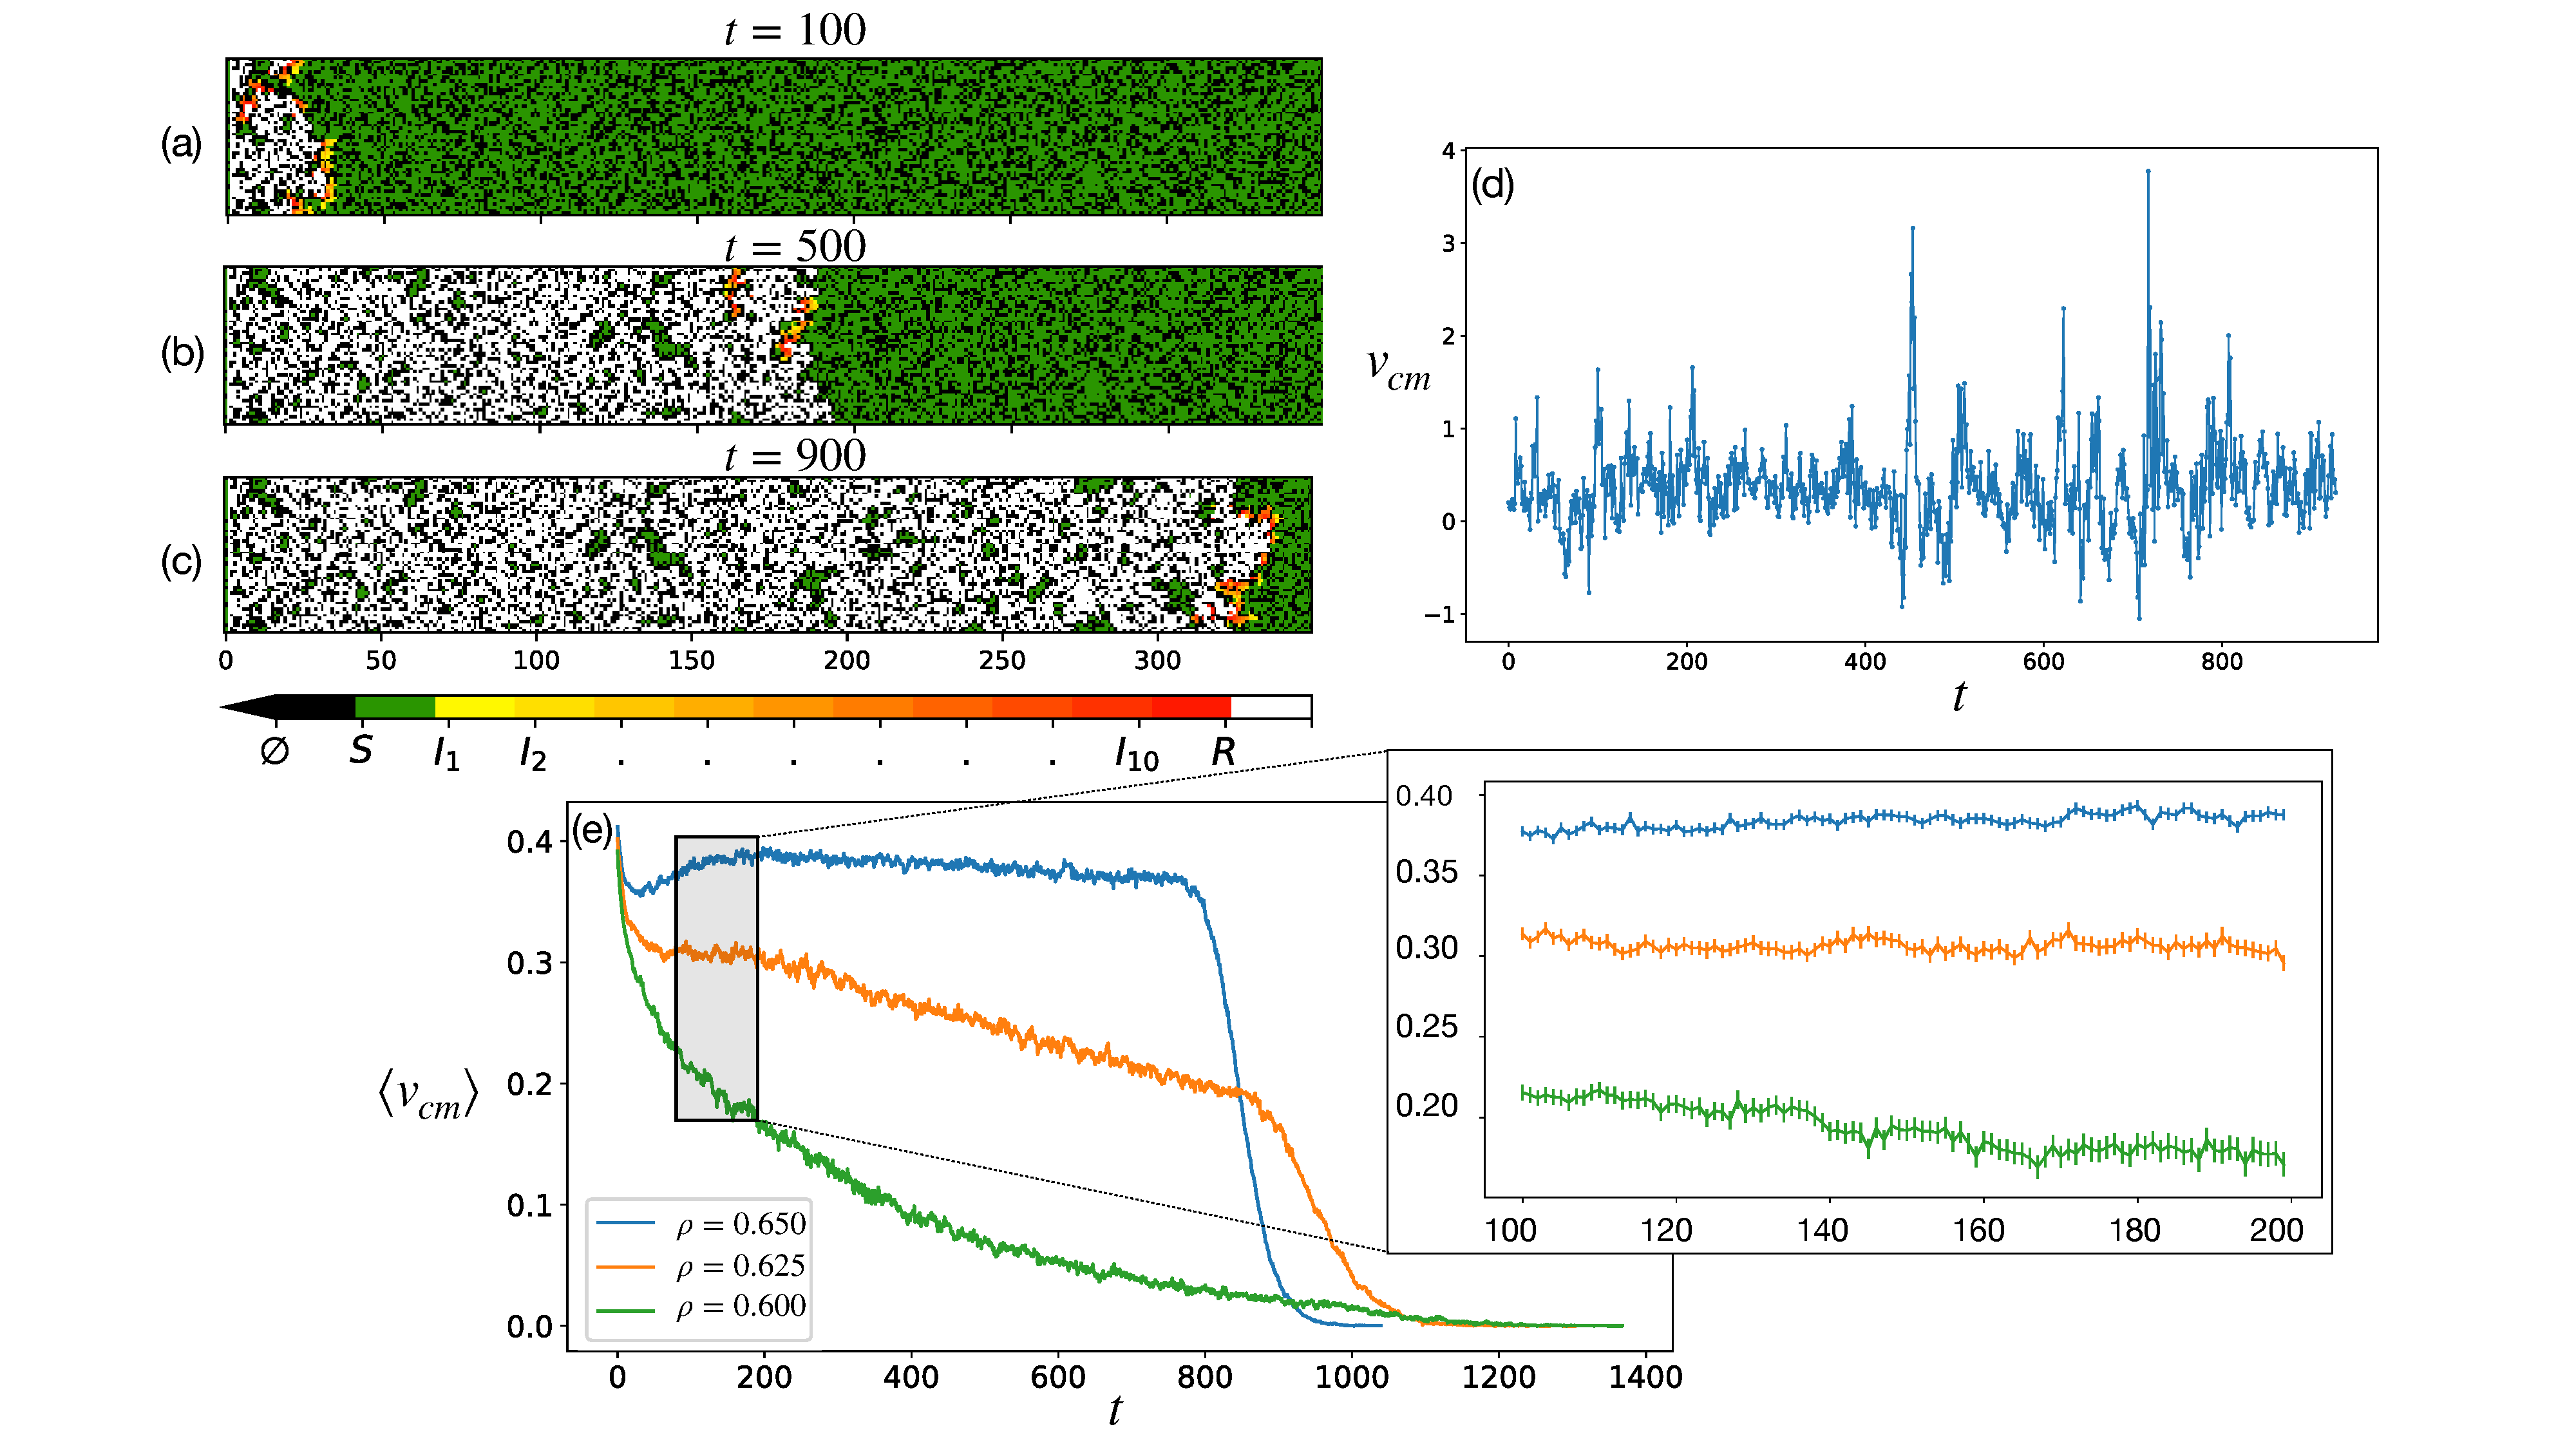
\includegraphics[scale=0.30]{chapter4/figures/figure1-channel-domain.pdf}
    \caption{
    (a-c) A channel domain of size $50\times350$ is shown over three time-steps for model parameters $\rho=0.65$ and $\beta=0.50$. 
    The center of infectious mass is recorded for each time-step. 
    (d) Plots of the center of mass time-series for the simulation illustrated in panels (a-c). 
    (e) The mean center of mass time-series (of $10^4$ repeats) for three variations in density and $\beta=0.50$. 
    Time-series begin to decay around the mean simulation run-time.  
    The zoomed inset shows the ensemble averaged time-series for $t\in[100, 200]$ and reveals increases in error bars lower density parameters.
    }
    \label{fig:ews-primer}
\end{figure}

\subsection{Centre of infectious mass}

The channel domain provides an advantageous setting to capture early warning signals, avoiding two-dimensional geometrical effects.
Moreover, the channel permits an improved (more intuitive) `centre of mass' metric (COM), based on the mean infectious tree displacement from the origin:
\begin{equation}
   v_{cm}(t) = \frac{\sum^i x_i(t)}{N_I(t)} - \frac{\sum^i x_i(t-1)}{N_I(t-1)}
   \label{eq:COM}
\end{equation}
where $x_i(t)$ is the spatial location along the $x$ axis of the $ith$ infected tree at 
time $t$ and $N_I(t)$ is the total number of infected trees at time-step $t$. 
 The form of Equation \ref{eq:COM} displays intrinsic similarities to the Newtonian center of mass:
 \[x_{cm} = \frac{\sum^i x_i\times m_i}{\sum_i m_i}\]
(where $m_i=1$ and $\sum^im_i= N_I$ in Equation \ref{eq:COM}).
Subsequently, COM velocity will denote the metric defined by Equation \ref{eq:COM}. 
Figure \ref{fig:ews-primer}(b) depicts the COM time-series corresponding to the simulation shown in Figure \ref{fig:ews-primer}(a). 
The COM time-series allows for negative values and looks different to those shown previously in Figure \ref{fig:vel_eff_rad_metric}(a).

Figure \ref{fig:ews-primer}(c) illustrates the COM ensemble-average, denoted by $\langle v_{cm}\rangle$, for the three values of tree density.
On average, the mean time series begins to decay after the mean lifetime of the simulation; the blue time-series shows a drastic decrease around $t \in [800, 900]$, which coincides with the pathogen reaching the domain boundary\textemdash also reflected in Figure \ref{fig:ews-primer}(c).
The green time series lies just above the threshold for percolation, and it decays more gradually $t=0$ because of the higher pathogen extinction probability. 
A small number of long-lasting simulations with run times exceeding $t>1000$ occurred in the green time-series, indicating criticality in the system\textemdash 
previously likened to a regime of persistence in section \ref{sec:SLM-epidemic-threshold}.
The inset of Figure \ref{fig:ews-primer}(c) shows the ensemble-averages between $t\in [100, 200]$, plotted beside the standard error for each time-step.
Error bars are most significant for the lowest-valued density shown in green, suggesting a more chaotic spread.
In principle, if the variance signature looks different before and after the epidemic regime, an early warning signal can be detected. 

\subsection{Ensemble averaging method}

An assessment of the temporal variability of the system is needed to detect an early warning signal. 
The findings of \cite{OROZCOFUENTES201912} were gathered by first producing a distribution of mean time-series velocities $\overline{v}_t$,
analogous to calculating variance, skewness and autocorrelation over the distributions of Figures \ref{fig:vel_eff_rad_metric}(b-d)
In this scheme, an early warning signal is detected from the variance of the mean velocity: $var\big\langle \overline{v}_t \big\rangle $.
Although assessing calculations based on the mean simulation variance, $ \big\langle \overline{var}({v}_t) \big\rangle $. revealed a clearer EWS.
We proceed by detailing an ensemble method that permits the capture of within-simulation variance. 

Before the ensemble averaging method is elaborated, it makes sense to define the relevant notion.
Suppose a simulation with parameters $\rho, \beta$ will last for $f$ time-steps, Equation \ref{eq:COM} describes the time series: $v_{cm}^{t=1}, v_{cm}^{t=2},..., v_{cm}^{t=f} \in V^{\rho\beta}$. 
Then, a set of independent time series can be generated by repeating $N$ simulations. 
A set of $N$ repeated simulations for an arbritrary point in the parameter-space ($\rho, \beta$) 
can be labelled as: \{$V_1^{\rho\beta}, V_2^{\rho \beta},..., V_N^{\rho\beta}\} \in \mathcal{V}_{\rho\beta}$, 
where each $V_i^{\rho\beta}$ describes an individual simulation time series and $\mathcal{V}_{\rho\beta}$ describes the entire ensemble for parameters $(\rho, \beta)$. 
Thus, an early warning signal is detected by calculating the mean time-series variance:
defined by:
\begin{equation}
\label{eq:ews_eq}
    \big\langle \overline{var}(v^{\rho\beta}_{cm}) \big\rangle = \frac{1}{N}\sum\limits_{i=1}^{N} var(V_i^{\rho\beta})
\end{equation}

To rigorously analyse an ensemble of time-series variances, 
we require the same number of observations within each ensemble. 
Otherwise, the classification of an early warning signal might be confused with statistical fluctuations and errors.
There are two observations to consider: 
A) the number of time steps within simulations, i.e. $v_{cm}^{t}$ 
B) the number of repeated simulations, $N$.
In general, stochasticity will prevent two simulations from having the same number of time steps, 
$|V_i^{\rho\beta}| \neq |V_j^{\rho\beta}|$.
Therefore, short-lived simulations with a small number of time steps might be more error-prone than long-lived simulations;
we introduce a fixed window of time-steps ($t_O\leq t \leq t_F$) to remedy this.
Provided the window length $t_F-t_O$ captures a sufficient number of time-steps, we avoid significant fluctuations in $V_i^{\rho\beta}$. 
Variance inside this window is defined by:

\begin{equation}
\label{eq:ews_eq1}
    \big\langle \overline{var}(v^{\rho\beta}_{cm}) \big\rangle = \frac{1}{N}\sum\limits_{i=1}^{N} var(V_i^{\rho\beta}\Big|^{t_F}_{t_O})
\end{equation}

Initial transience constrains the particular choice of $t_O$ in the channel domain, 
which could, in principle, distort calculations of the time-series variance\textemdash 
analogously presented when discussing Figure \ref{fig:vel_eff_rad_metric}(a). 
We set $t_0=100$, as initial instability occurred most over the first $100$ time-steps 
(as shown in Figure \ref{fig:ews-primer}(e), particularly by the blue time series). 

Neglecting the first $100$ time steps helps limit the initial transience,
although it introduces an additional complication.
Namely, if we do not include simulations with less than $t_O=100$ steps, some ensembles $\mathcal{V}_{\rho\beta}$ % 
might comprise less than $N$ variance observations;
an ensemble mean might therefore be more error-prone and lead to misclassified EWS.
In a similar vein, if the value of $t_F$ is too high, a large proportion of simulations might not survive to give $N$ measures of variance. 

Unfortunately, the criterion of measuring simulation variance in the window $[t_O, t_F]$ 
and capturing all $N$ observations is infeasible, mainly when parameters are low, e.g. the trivial case of $\rho=0$ and $\beta=0$.
Fortunately, however, an early warning signal is only detectable immediately before 
and after the epidemic threshold; other parameter space regions are less important.
Thus, if the relevant regions in parameter space survive long enough to measure variance in the window $t \in [t_O, t_F]$, 
we may confidently detect an early warning signal.
Given the above concern, we chose $t_F = 200$; 
this struck the best balance between avoiding initial transience and ensuring the maximum possible number of simulations 
survive long enough to calculate variance over a sufficient window.


\subsection{EWS parameter-sweeps}
\label{section:ews_slm}

Figure \ref{fig:ews-results} displays the mean time-series variance, as per Equation \ref{eq:ews_eq1}.
The colour bar shows variance over the entire parameter space of density and infectivity from white to back.
In Figure \ref{fig:ews-results}, the lower and upper red lines indicate a percolation probability of $Pr(\rho, \beta)=0.05$ and $Pr(\rho, \beta)=0.95$, respectively.
Inside these regions, the system transitions into an epidemic and we witness a considerable rise in the variance.

The observations of Figure \ref{fig:ews-results} agree with the results of \cite{OROZCOFUENTES201912}. 
Interestingly, measuring EWS over a two-dimensional parameter space reveals that some values 
of $\rho, \beta$ preempt the epidemic by a larger margin\textemdash indicated by the red 
arrows. 
Precisely, this occurs for a lower infectivity 
($\beta<0.40$) and higher density. 

\newpage

 \begin{figure}
    \centering
    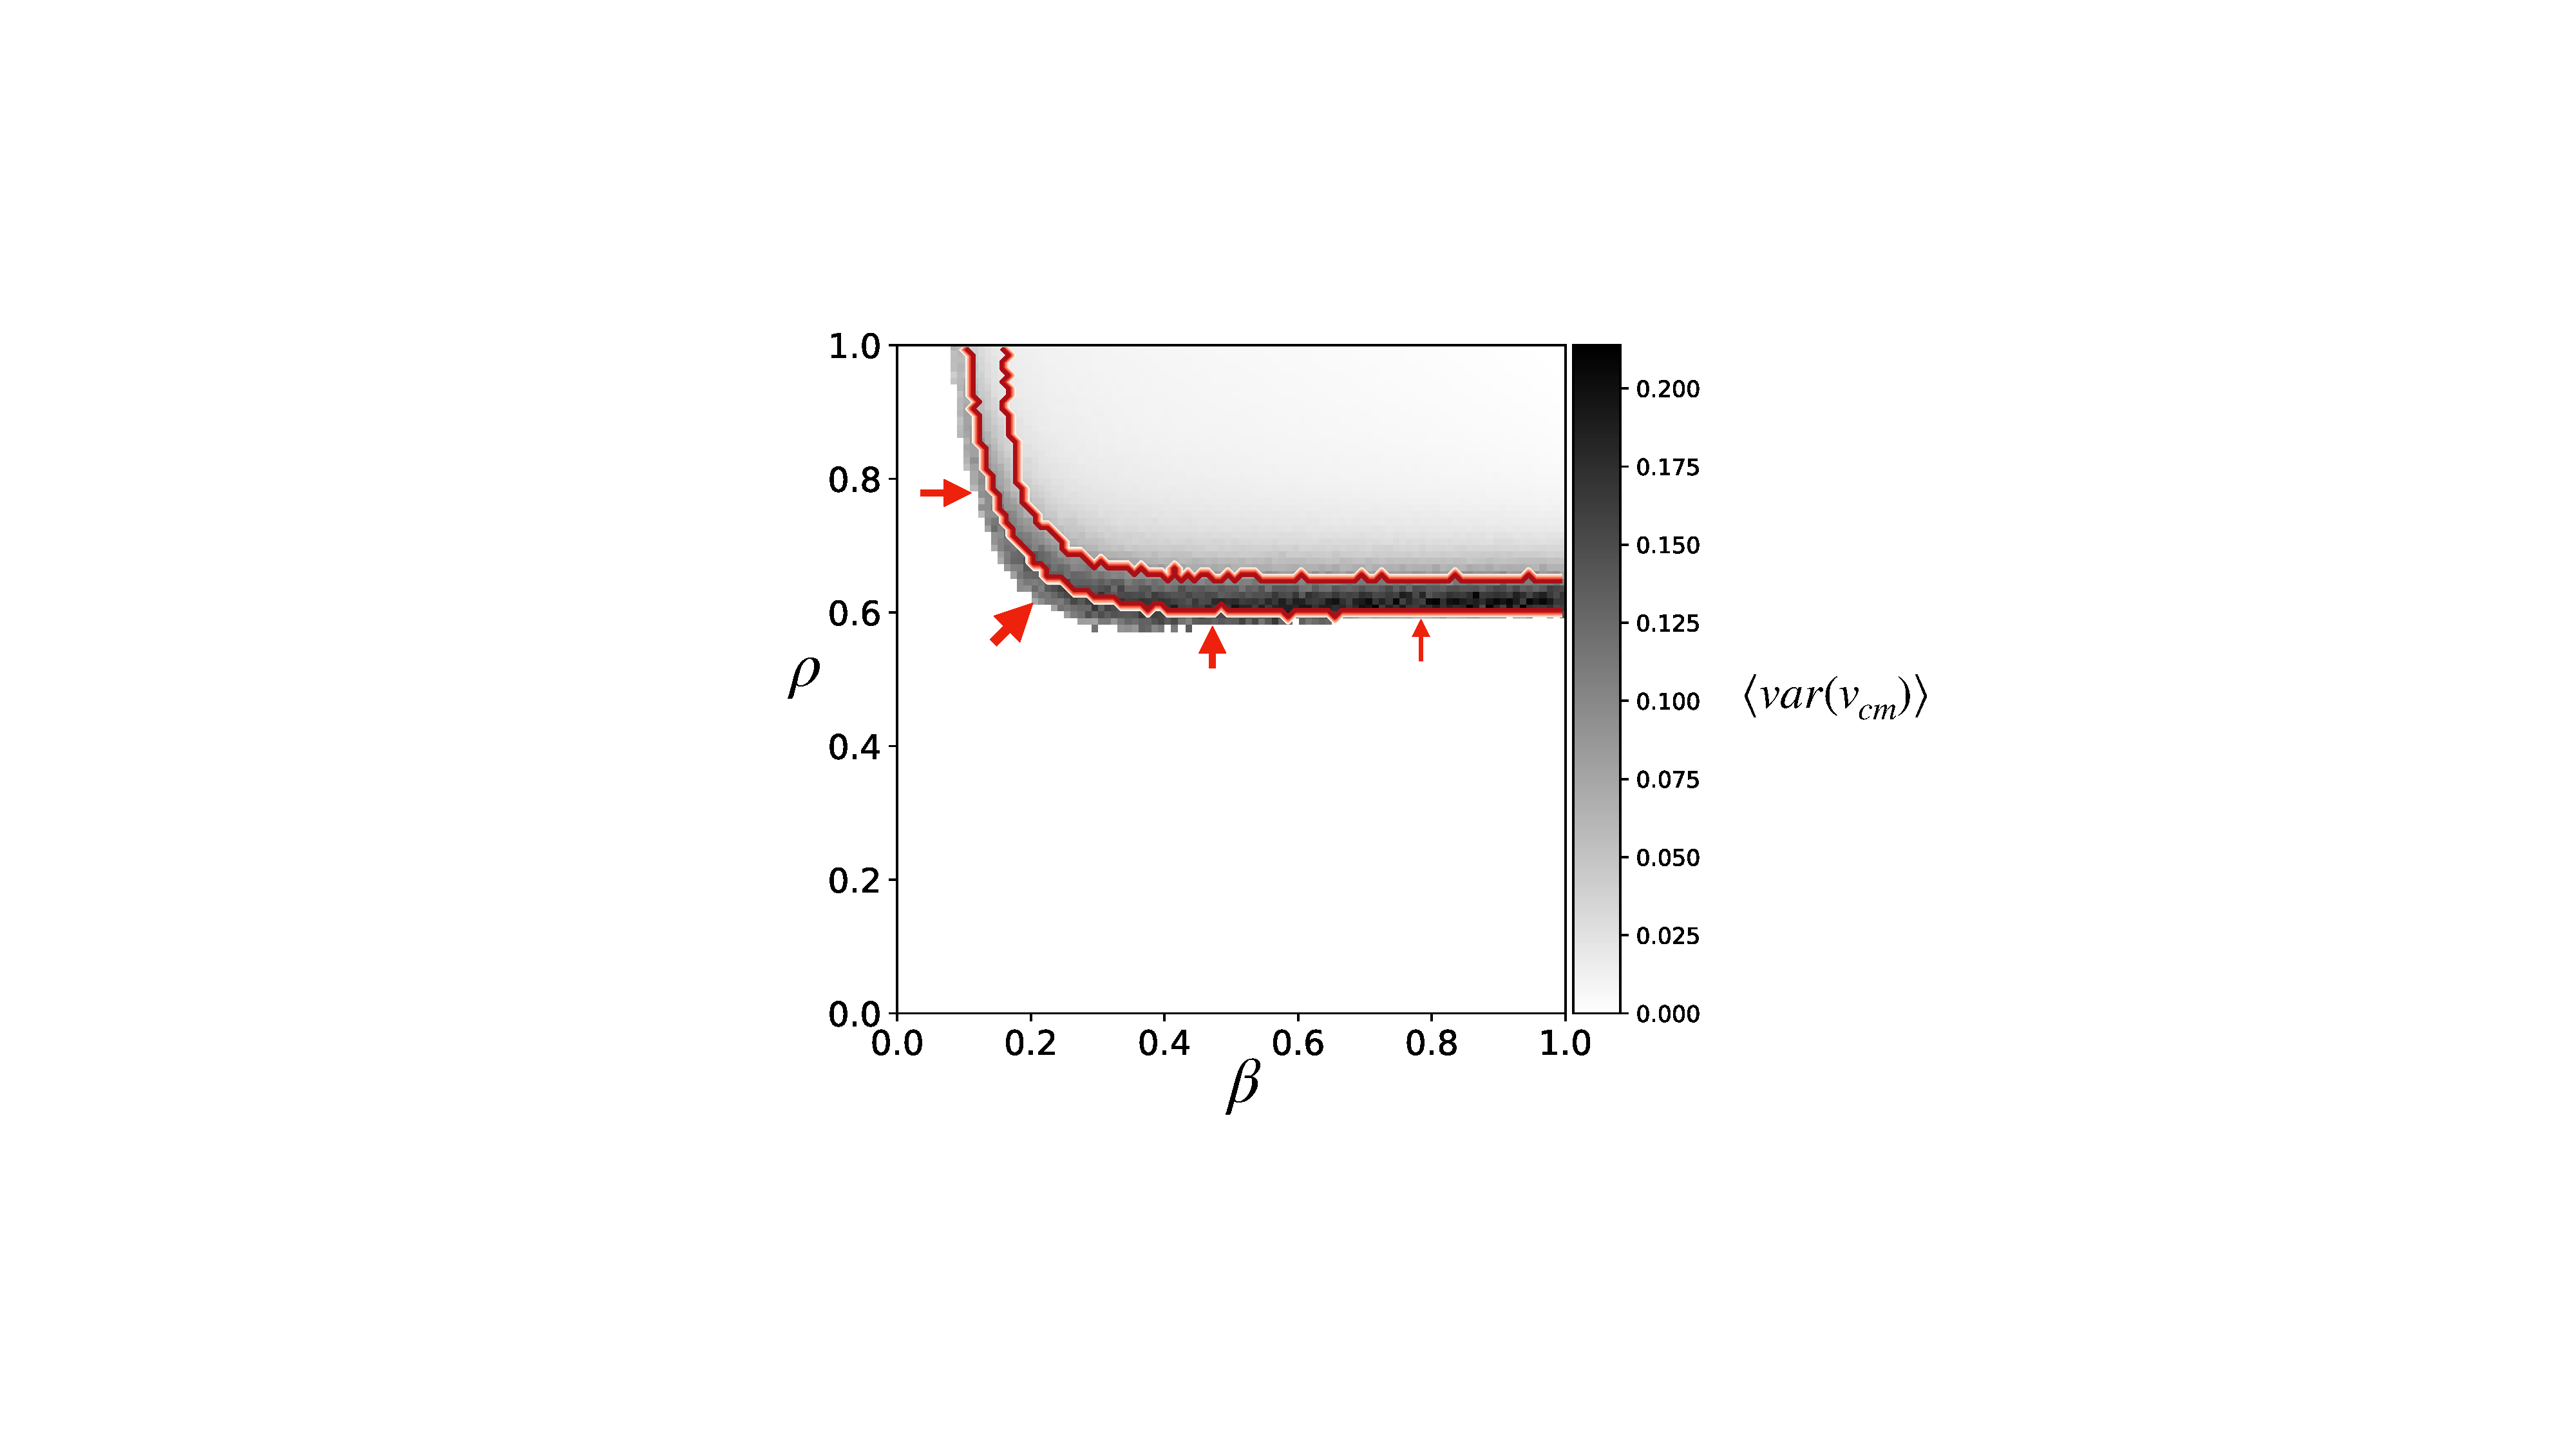
\includegraphics[scale=0.45]{chapter3/figures/figure11.pdf}
    \caption{The ensemble-averaged variance of $v_{cm}(t)$ over a two dimensional parameter sweep of $\rho$ and $\beta$. Red contours show the lower and upper bound of percolation (i.e. between $5\%$ and $95\%$ probability). 
     The epidemic regime is preempted by increases in variance more clearly for certain parameter values, %
     indicated by the arrows.}
    \label{fig:ews-results} 
\end{figure}

The following thought experiment can explain the EWS asymmetries in Figure \ref{fig:ews-results}: %
suppose infectivity is high, and density lies just below criticality ($\rho\lesssim\rho_c$), 
so susceptible clusters do not percolate. 
In this case, disease transmission is high on account of $\beta$, 
and all susceptible hosts become quickly infected, 
although an outbreak will come to a halt due to insufficient hosts. Therefore, in this model, 
an aggressive pathogen spreading through low tree densities may propagate rapidly but have a short, 
chaotic signature. Hence the transition is steep,
and the simulation variance is significant, as indicated by the smallest arrow in Figure \ref{fig:ews-results}. 
In this region, detecting an EWS is hard because transitions occur most rapidly.

Now consider the converse, a less infectious pathogen with an abundance of susceptible hosts, 
located in the top-left region of Figure \ref{fig:ews-results}.
Here, transitions into the $I$ compartment are slower because the pathogen is less infectious, 
although this time, hosts are abundant.
Thus, a pathogen is likely to spread predictably for longer times, 
giving rise to a slightly less abrupt variance signature, 
as indicated by a lighter colour before the transition in the top left quadrant of Figure \ref{fig:ews-primer}.
Although the variance spike is not as significant, 
it preempts the epidemic transition by a more considerable degree\textemdash
indicated by the larger arrows in Figure \ref{fig:ews-results}.
Altogether, Figure \ref{fig:ews-results} suggests that EWS strength depends on the particular combination of epidemic parameters; 
although fundamentally, an EWS is detectable for all parameter combinations/

\newpage


\section{Modelling with realistic geometries}

% JS_Another thought experiment as in the previous chapter? - This is lazy just consider this properly and formally.

Consider a single source of infestation located at the center of a regular square domain. %
The number of the infected-dead trees which result from an outbreak is determined. %
Then the boundary of the square domain is randomly deformed such that a complicated irregular %
shape is realised and  the epicenter is arbitrarily re-positioned  to a different position. %
From this, it is clear to see that the total number of infected-removed trees is going to be different from the regular-isotropic scenario. %
Therefore, we assume \textit{a priori} that a complicated geometry can alter both the threshold and how the dynamic behaviour of the disease progression is defined. %

Using the same $SIR$ compartments and model dynamics to those presented in Chapter \ref{chapter:SLM}, %
we move onto a map of Great Britain. As a first step, only the coastline of Great Britain will be explored. %
That is, the introduction of a complicated geometrical boundary or edge. %
Figure \ref{fig:uk-spread-primer} shows an outline of Great Britain (GB) filled with a random homogeneous distribution of land `patches' at resolution $1\mathrm{km^2}$. %
Green represents susceptible patches and black represents insusceptible\textemdash as explained in the previous Chapter for trees a unit hosts. %

It is clear that edge effects will reduce the probability of an epidemic when the source %
of infection is at the coast or close to the boarder of an island such as GB. %
Depending on the level of geographical %
regularity, the local fractal dimension of the coastline will vary. %
The more irregular the portion of coastline, the closer the fractal dimension will approach $2$. %
Whereas, a perfectly straight coastline will have a fractal dimension of $1$. An example of %
how edge effects may alter the spread of disease is shown in the inset of Figure \ref{fig:uk-spread-primer}. %
An epicenter just below the Humber estuary is thought to pose less risk on account of the discontinuity between landmass. %

If an epicenter is located on the boundary of an irregular coastline, pathogen-impedance %
will be high and the risk of epidemic reduced. If, on the other hand, an epicenter was located inland, %
the effects of an irregular coastline become negligible. %

To study  edge effects of the coastline and map-geometry, each lattice site $(i, j)$ inside %
the landmass (denoted by $\in \mathcal{L}_{GB}$) is taken as a potential epicenter. %

A simulation can then iterate through each lattice point $(i,j)$ where the infection will be %
allowed to evolve through the domain and the number of removed patches will be recorded. %
A measure of the scale of epidemic through each epicenter can be summarised by a metric of the form: %
\begin{equation}
\label{eq:epi_impact}
    \chi=\frac{|R|}{S_0}
\end{equation}
where $|R|$ is the number of patches in the removed state and $S_0$ is the number of susceptible %
patches at time $T=0$. Here, $\chi$ represents a naive indicator of \textit{tree-mortality} %
and by extension `\textit{epidemic-impact}'. The measure $\chi$ will be refereed to as mortality %
ratio from now on. %

\begin{figure}
    \centering
    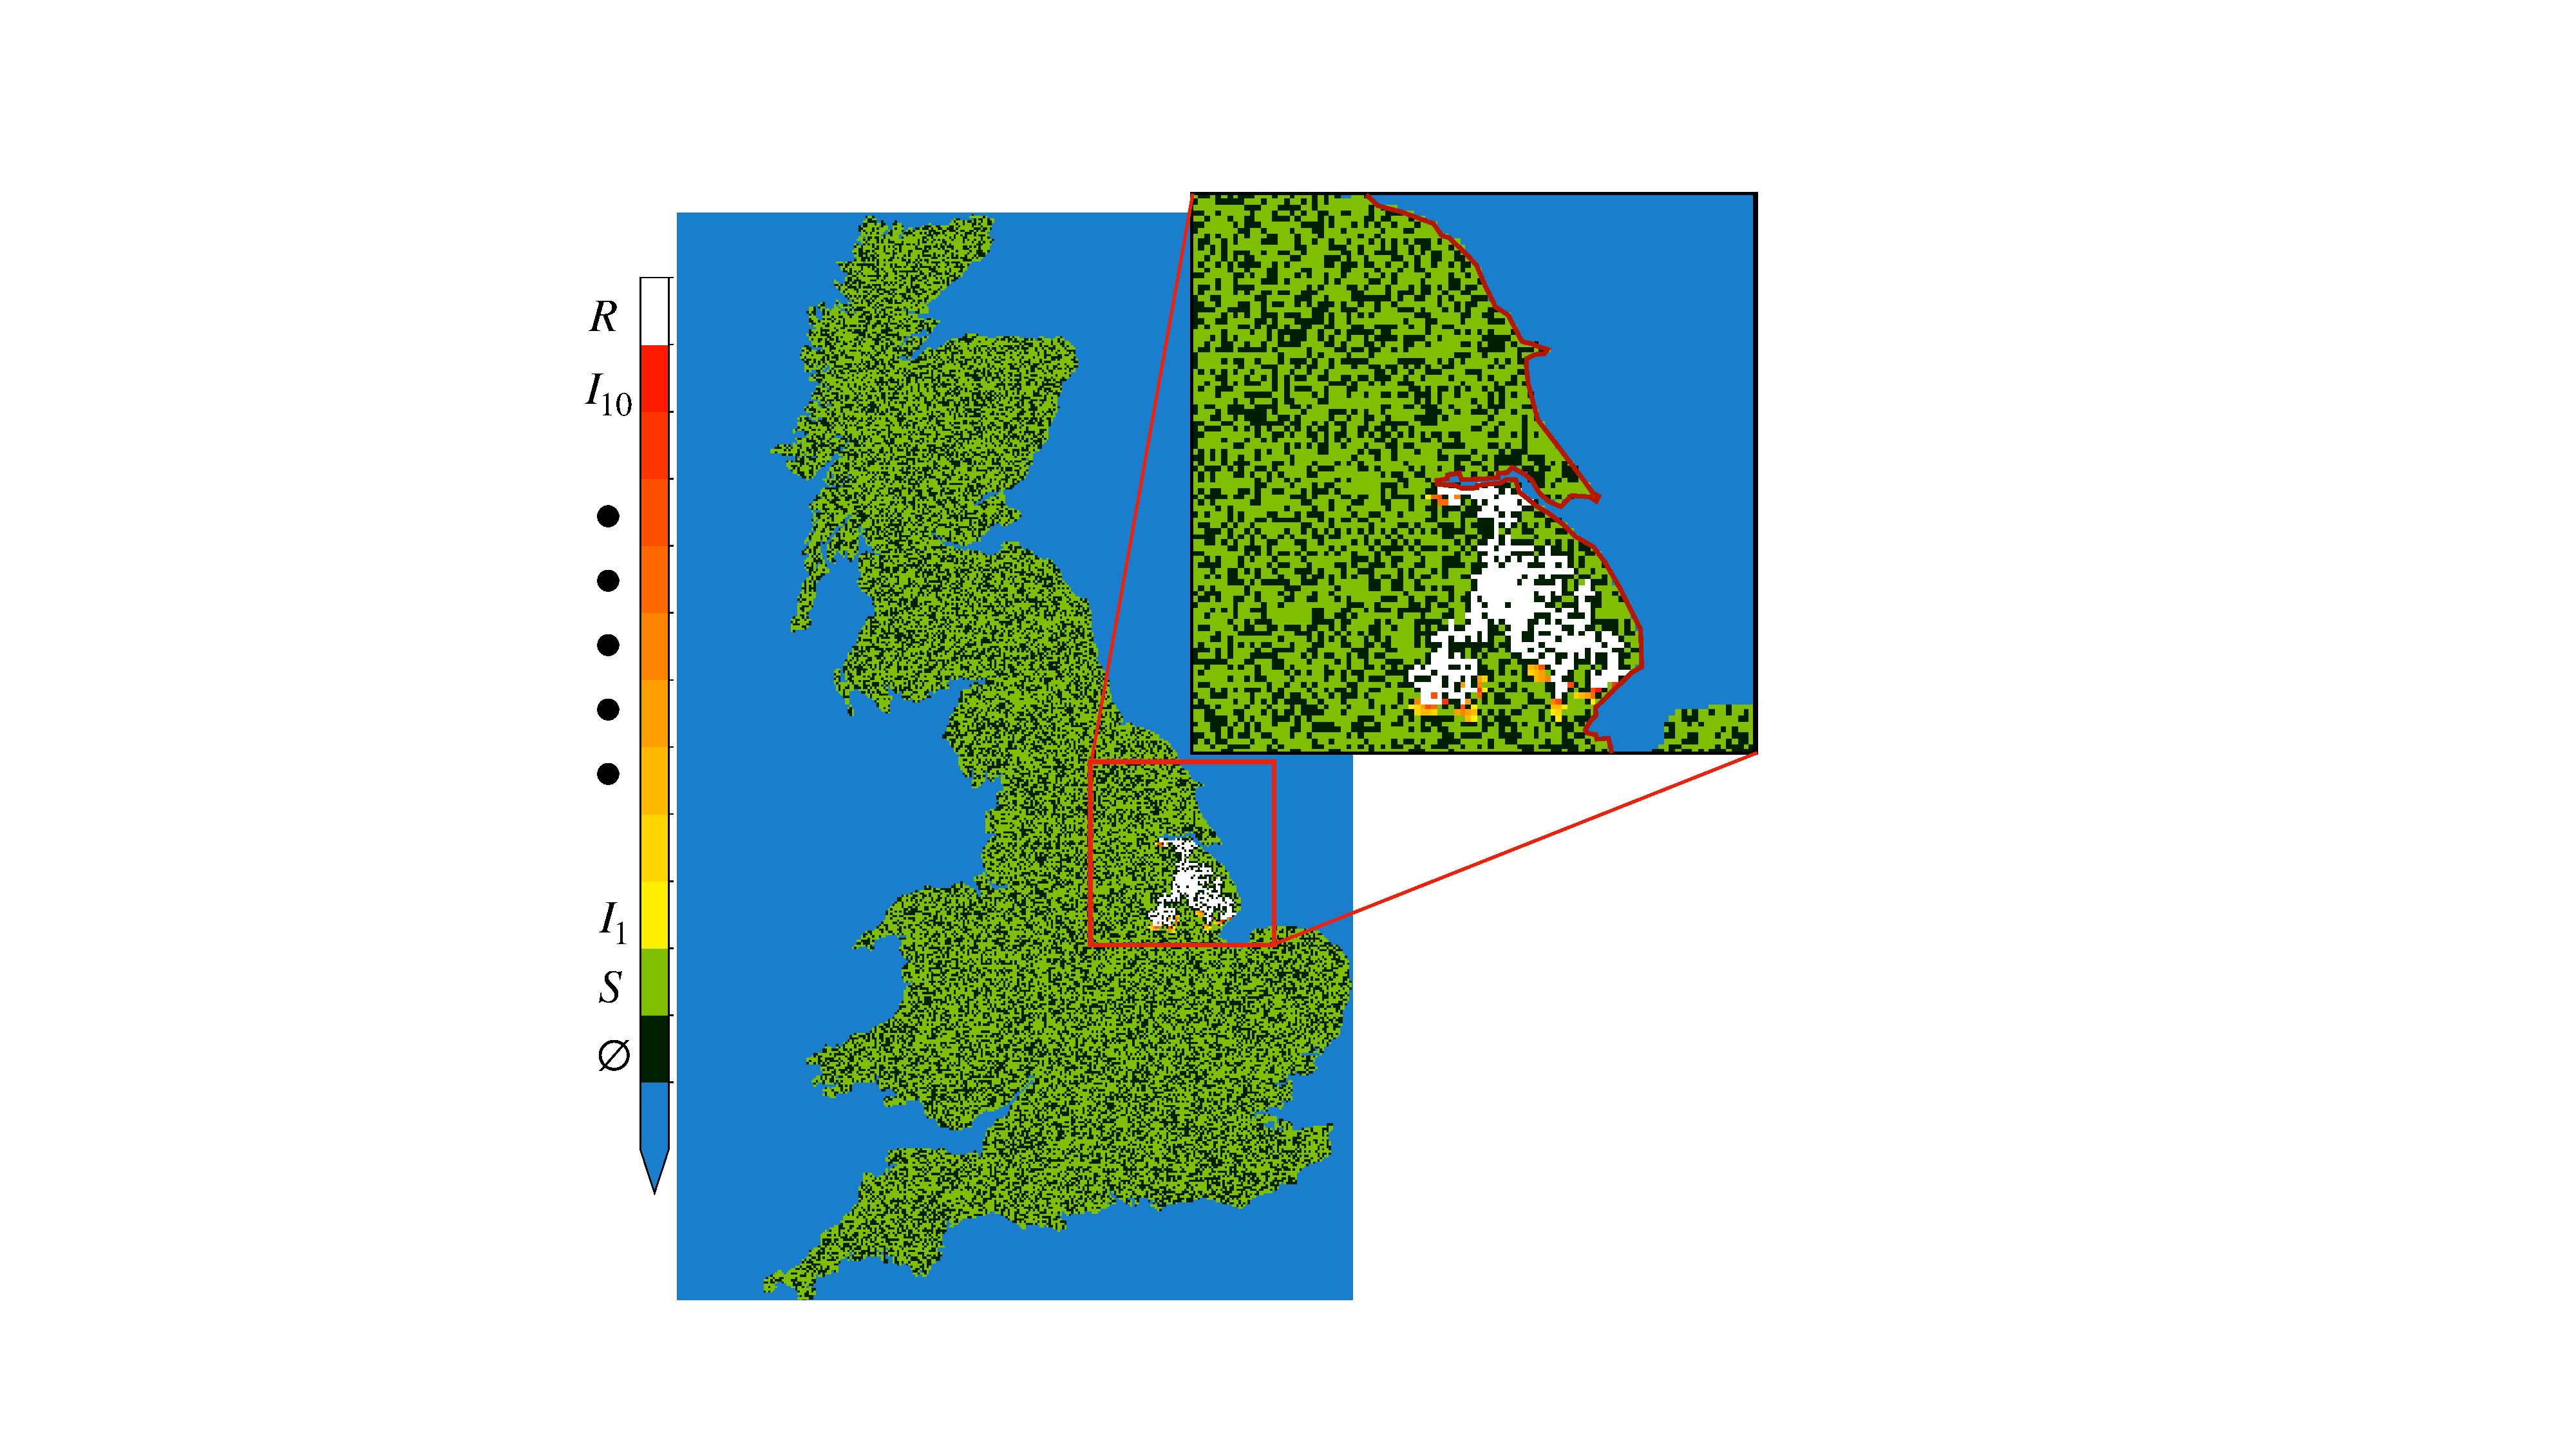
\includegraphics[scale=0.3]{chapter4/figures/figure1.pdf}
    \caption{The simple lattice model spreading on a map of GB. Lattice geometry and epicenter %
    location are non-trivial aspects likely to influence the spread of disease. The zoomed inset %
    shows an example of the Humber estuary preceding an infectious wave-front. }
    \label{fig:uk-spread-primer}
\end{figure}

% Introduce simulation run-time and mortality. Show epicenter variations
\begin{figure}
    \centering
    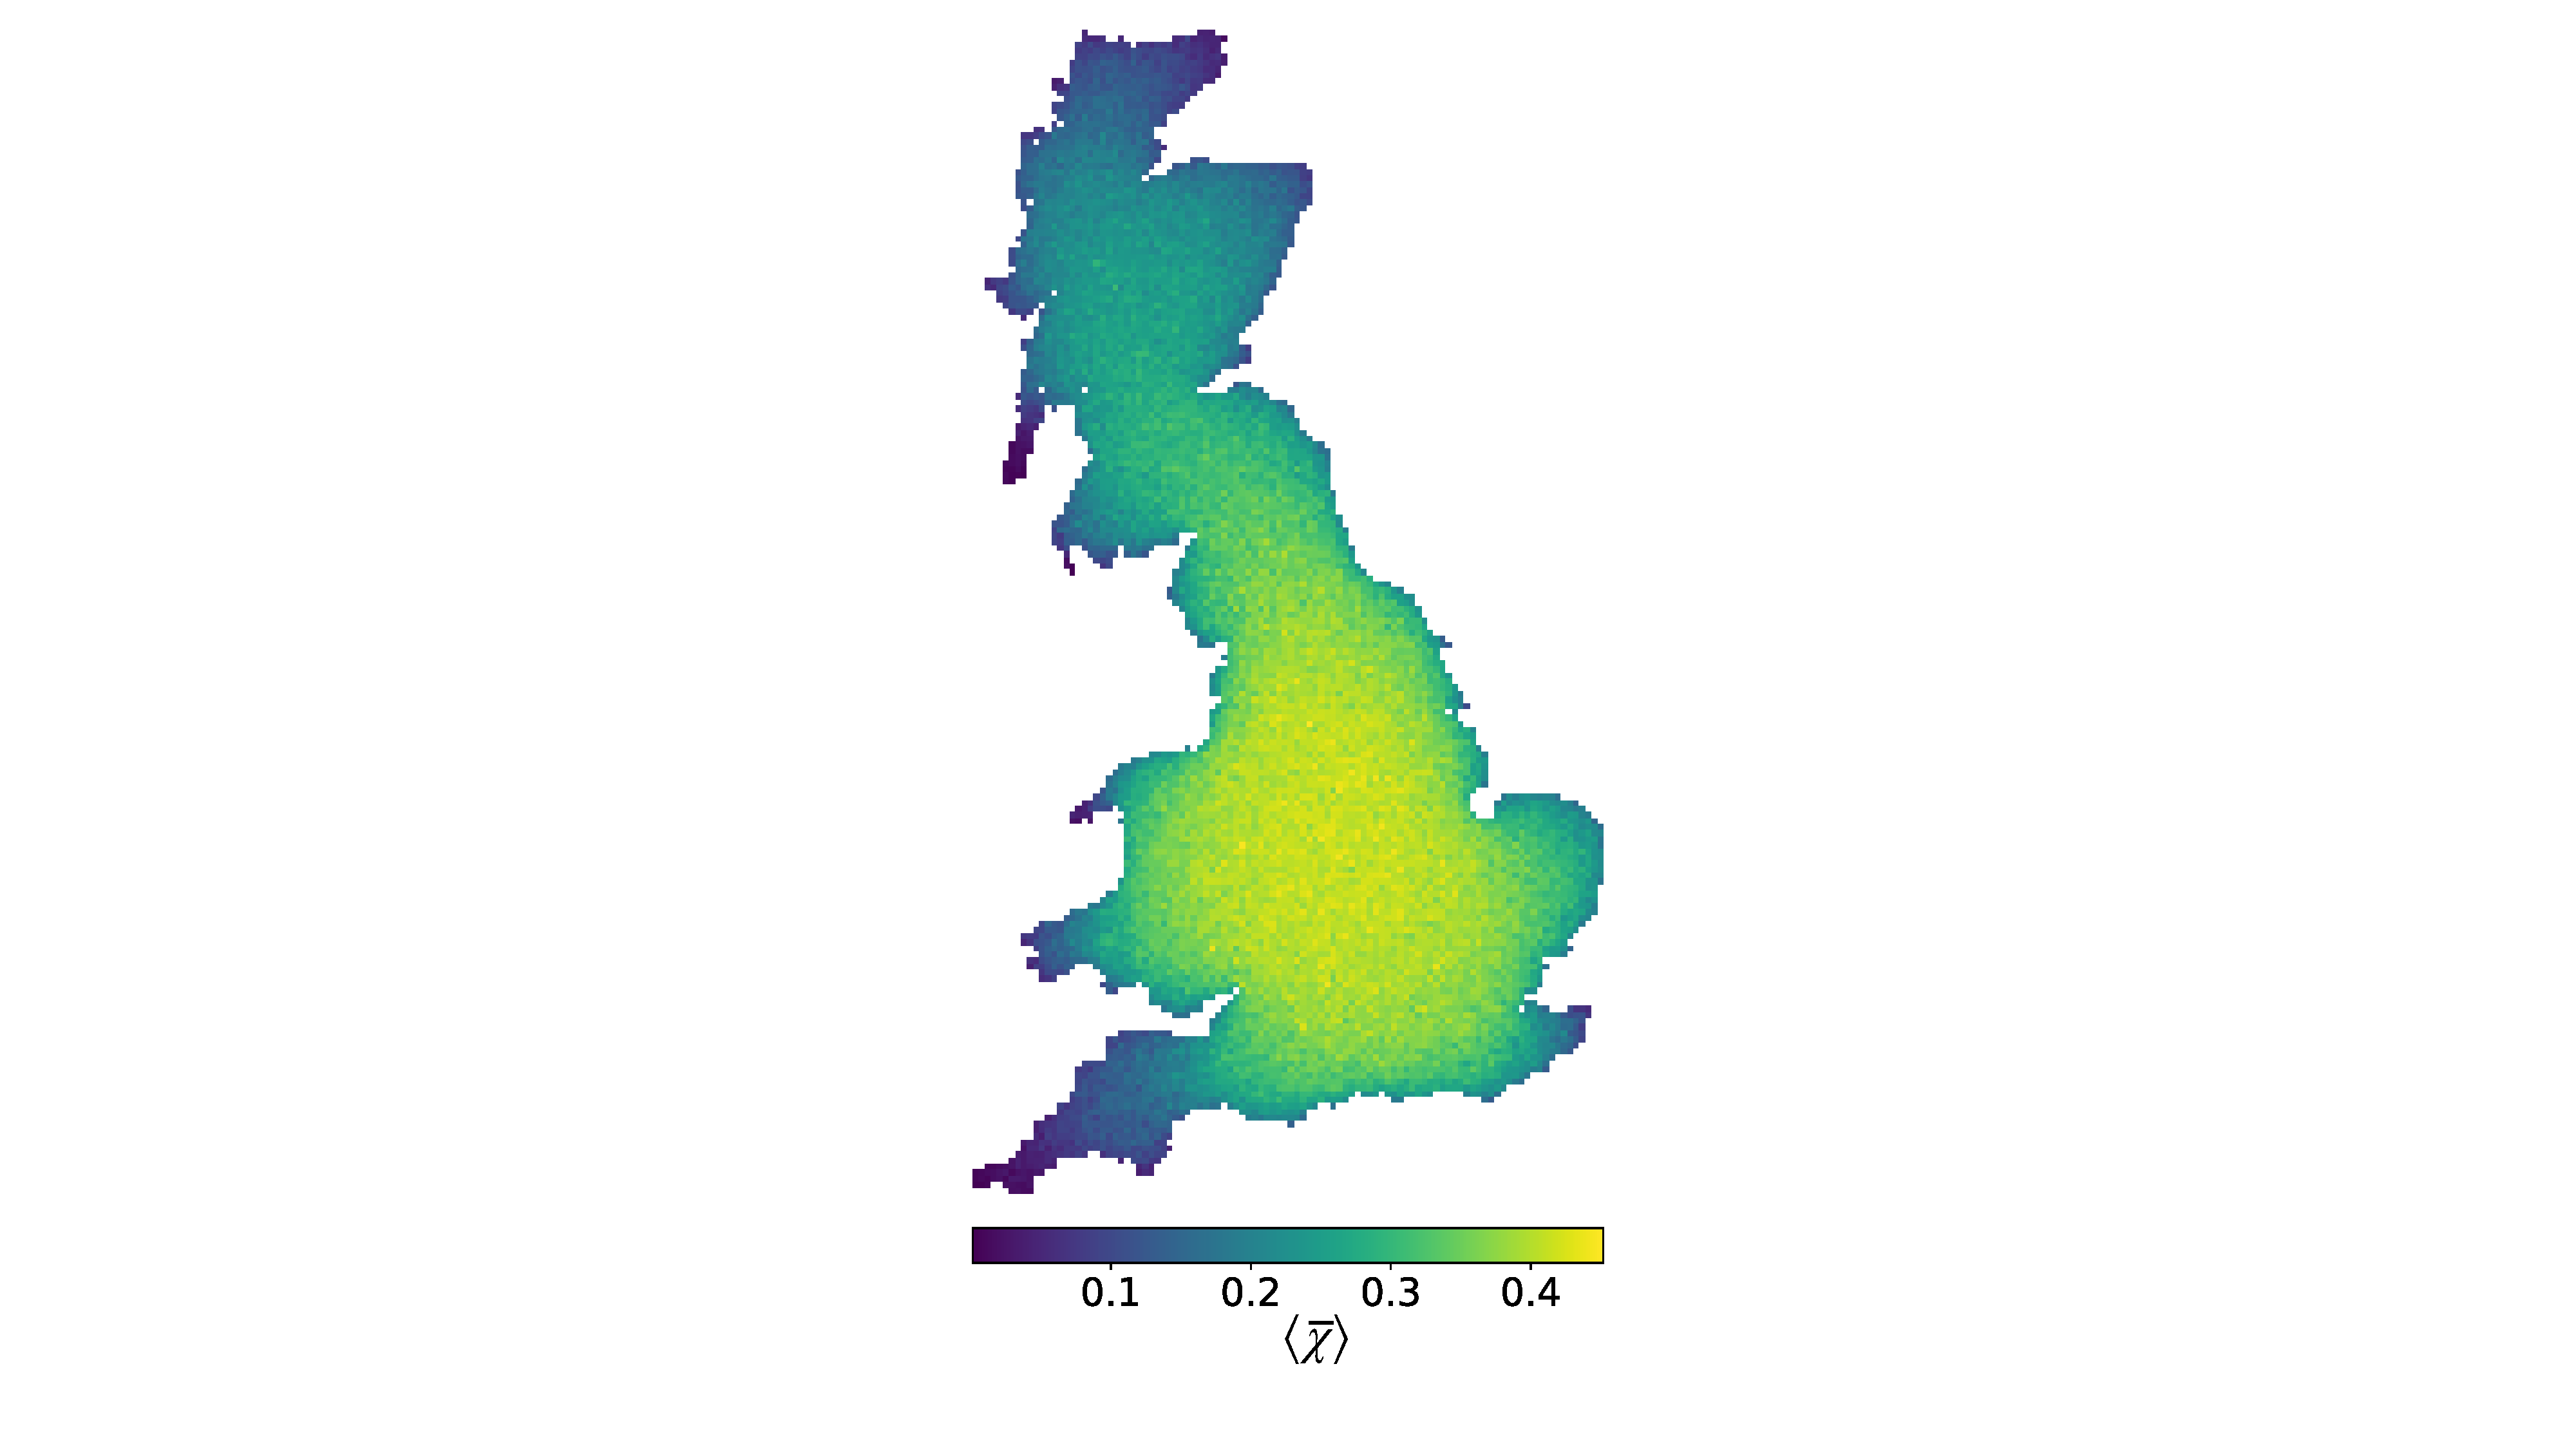
\includegraphics[scale=0.32]{chapter4/figures/figure2.pdf}
    \caption{Each pixel in the domain is treated as an epicenter and averaged over an ensemble. %
    Color shows the mortality ratio $\chi$ for each spatial location and demonstrates edge effects %
    in a complicated landscape.}
    \label{fig:uk-spatial-risk}
\end{figure}

Given the system stochasticity, it is necessary to repeat simulations for each epicenter %
and calculate $\overline{\chi}$. Iterating over the whole of the GB in this way allows us 
to visualise the spatial-susceptibility of the pathogen $\beta$. %
The value of spatial-susceptibility depends on both $\rho$ and $\beta$ and forms a primitive %
notion of risk within the toy-model. %

Figure \ref{fig:uk-spatial-risk} shows the result of ensemble averaging $\chi$ for each %
patch of land\footnote{Ensemble averaging each patch of land is computationally intensive. %
To account for this domain shown in \ref{fig:uk-spread-primer} was coarse-grained to a resolution of $5\mathrm{km^2}$. %
Simulations were conducted on the Leeds high-performance computing facility, the ARC-HPC system. %
The simulations shown in Figure \ref{fig:uk-spatial-risk} were ensemble-averaged using a task %
array and had a run-time of two hours (Repeated once per core, using $25$ cores).} %

The SLM assumed parameter values of $\rho=0.65$ and $\beta=0.25$ (just above threshold in a $2D$ square lattice). %
As expected, regions close to the edge are unlikely to result in a large epidemic. %
The narrow width across the Anglo-Scottish boarder reduces the mortality. %
Centralised regions show a roughly constant susceptibility. %

The method presented to assess spatial susceptibility, combining ensemble-averaging and %
spatially iterations for distinct land-points, will be frequented throughout the thesis. %

\section{Introducing realistic host data}

So far, this work has concentrated on a random homogeneous distribution of hosts. %
We now consider what changes occur for more realistic heterogeneous distributions. %
In ecology, collecting high quality data is time consuming and expensive. %
As remarked in Section \ref{chapter2:plant-ecologoy}, sampling a species to generate host %
data over an entire country is unfeasible. %
To account for this, an inferred data-set of common Oak (\textit{Quercus robur}) is used, %
as reported by \cite{hill.data}. %
This will couple the toy-model to a heterogeneous data-set and allow us to explore some %
fundamentally different properties. %
 
The distribution of Oak data is shown in Figure \ref{fig:uk-oak-l.hill}(a) along with its 
probability density function in  Figure \ref{fig:uk-oak-l.hill}(b). %
The units are hectares of canopy cover per kilometer squared of land, $\mathrm{ha/km^{2}}$. %
This is a convenient choice given $\mathrm{1\ ha = 0.01\ km^2}$. Each measure of abundance %
value can therefore be seen as a `percentage' of cover per land-point. %
The Abundance canopy cover, denoted by $\rho$, is shown in \ref{fig:uk-oak-l.hill}(a) as colour. %
As we can see, the spatial map now displays strong irregularities and host heterogeneity is visible. %

The probability density function, $f(\rho)$, is shown in Figure \ref{fig:uk-oak-l.hill}(b) and %
reveals that most land patches occupy a lower canopy cover values. %
The distribution had a small number ($\sim 5\%$) of outlying host abundance values%
 $10<\rho<35\ \mathrm{ha/km^2}$ which skewed the distribution. %
 These were reduced to $10\mathrm{ha/km^2}$ thus capping the highest value of $10\%$ canopy cover. %
 
The Oak data-source presents a problem when one recounts the SLM host-densities lay in the %
interval $\in [0, 1]$. Additionally, for each value of density, the SLM  assumed a binary %
valued domain with susceptible and empty lattice points. %
This is contrary to Figure \ref{fig:uk-oak-l.hill}. %

\begin{figure}
    \centering
    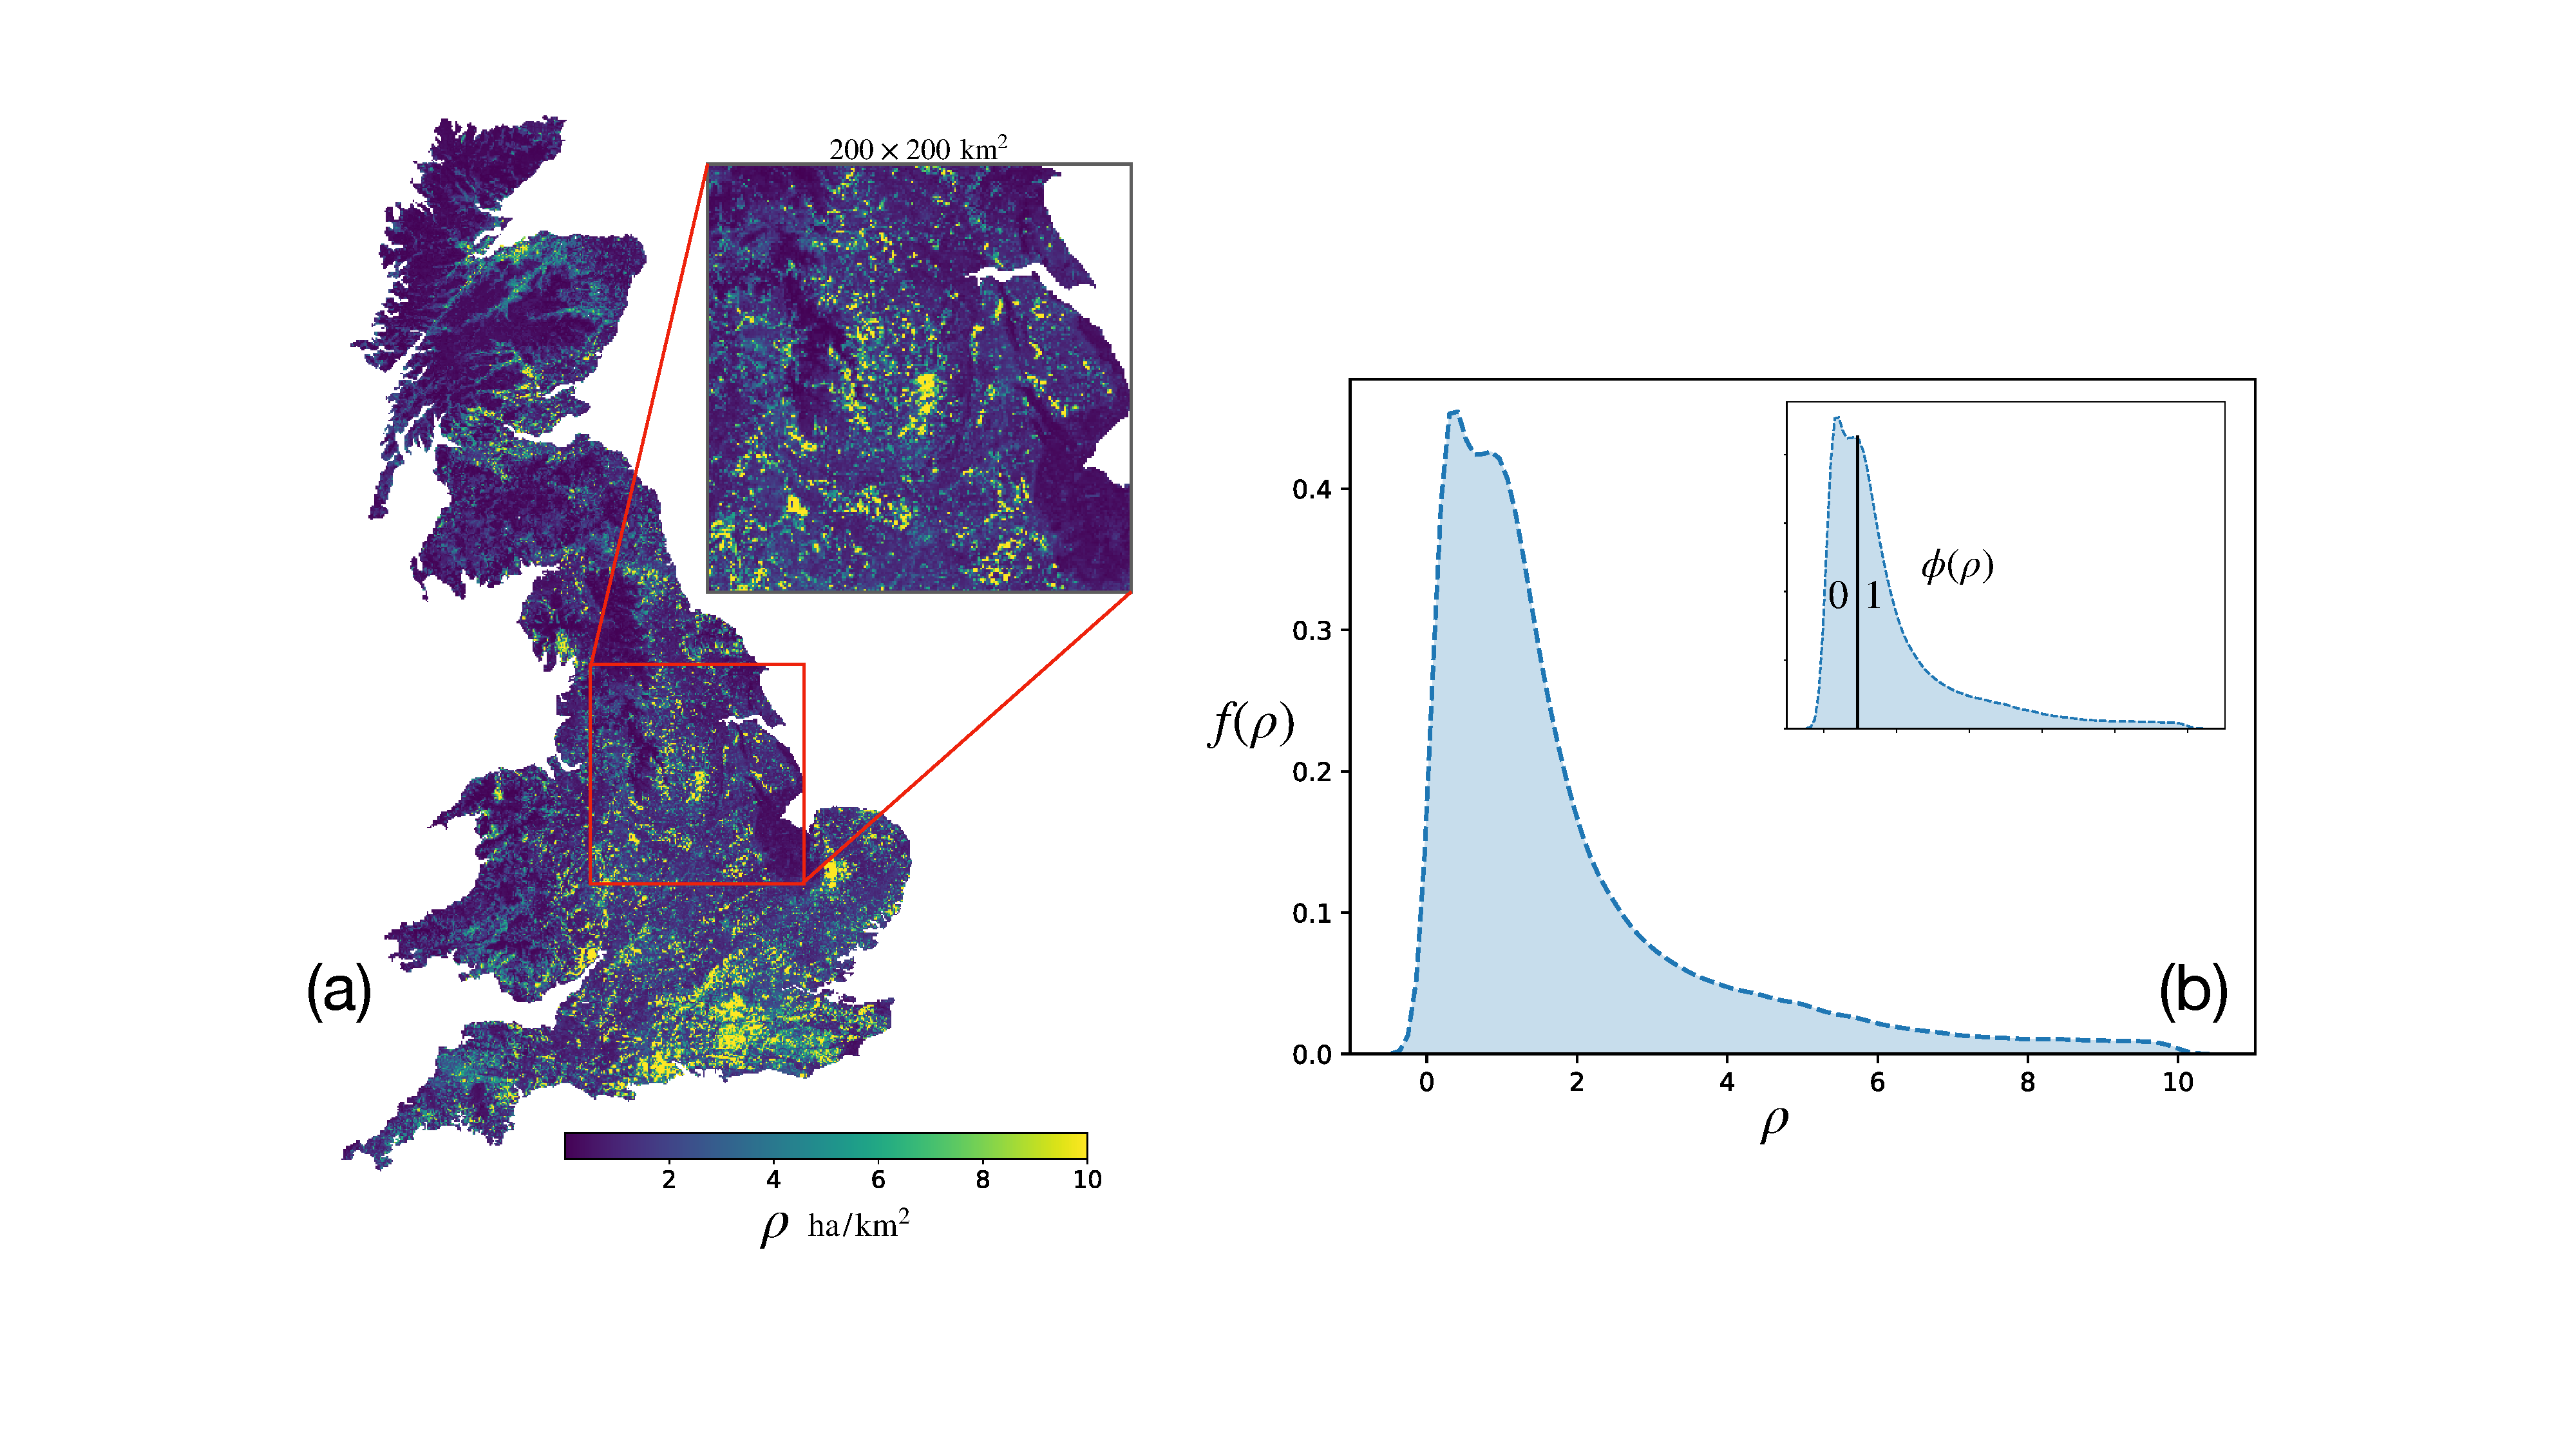
\includegraphics[scale=0.32]{chapter4/figures/figure3.pdf}
    \caption{(a) The modelled abundance distribution of common oak (\textit{Quercus robur}), inferred by \cite{hill.data}. The each pixel holds a predicted value of abundance having units hectares of canopy cover per kilometer squared of land. (b) The probability density function of abundance $f(\rho)$. The zoomed inset illustrates the process of generating threshold function $\phi$.}
    \label{fig:uk-oak-l.hill}
\end{figure}

In order to account for this, a threshold function $\phi(\rho)$, is introduced and defined by:
\begin{equation*}
  \phi(\rho) =
  \begin{cases}
    1 & \rho_{i,j}\geq\rho \\
    0 & \rho_{i,j}<\rho
  \end{cases}
\end{equation*}
for each continuous value of abundance, $\rho\in[0, 10]\ \mathrm{ha/km^{2}}$, the function %
 $\phi$ converts a patch of land $(i,j)$ into a binary value of one if it is greater than or %
 equal to $\rho$, otherwise zero. %
 This generates a binary-valued domain with susceptible $S$ when $\rho_{i,j} > \rho$ and %
 insusceptible $\emptyset$ when $\rho_{i,j} < \rho$. This idea is captured on the inset of %
 Figure \ref{fig:uk-oak-l.hill}(b), the vertical black line is an arbitrary threshold of %
 density $\rho$, where all canopy cover values less than $\rho$ are taken as insusceptible %
 with numerical value $0$. Whereas, all patches of canopy cover in the data equal to or greater %
 than $\rho$ are taken as susceptible and take the value $1$. In this picture, susceptible %
 land-patches have enough Oak trees to support the survival, growth and spread of disease. %
 Patches of land below the abundance threshold are presumed insusceptible and have an insufficient %
 number of hosts to survive and reproduce. %

In chapter \ref{chapter:SLM}, a distribution of hosts were easily characterised with $\rho$. %
Now however, heterogeneity in the data prevents a simple description of density. %
To overcome this one can define an \textit{`effective'} domain density, denoted by $\rho^*$,  by considering the percentage of susceptible land inside the domain:
\begin{equation}
    \label{eq:rho_eff}
  \rho^{*} = \frac{\sum^{i, j} ( \rho_{i,j} \geq \rho )}{|\mathcal{L}_{GB}|}
\end{equation}
where $\mathcal{L}_{GB}$ represents host distribution over Great Britain. %
 The terms $\sum^{i, j} (\rho_{i,j} \geq \rho)$ and $|\mathcal{L}_{GB}|$ therefore represent %
 the total number of susceptible patches and total landmass respectively. %

Given an increase in the susceptibility threshold $\rho$, the %
 effective density $\rho^*$ decreases. % 
However, a  decrease in the threshold $\rho$ increases $\rho^*$ as more patches become susceptible. %
The effective density $\rho^{*}$ therefore presents a convenient, although primitive, proxy %
for the density of host occupation over a heterogeneous distribution. %

\subsection{Epidemics through heterogeneous landscapes}
\begin{figure}
    \centering
    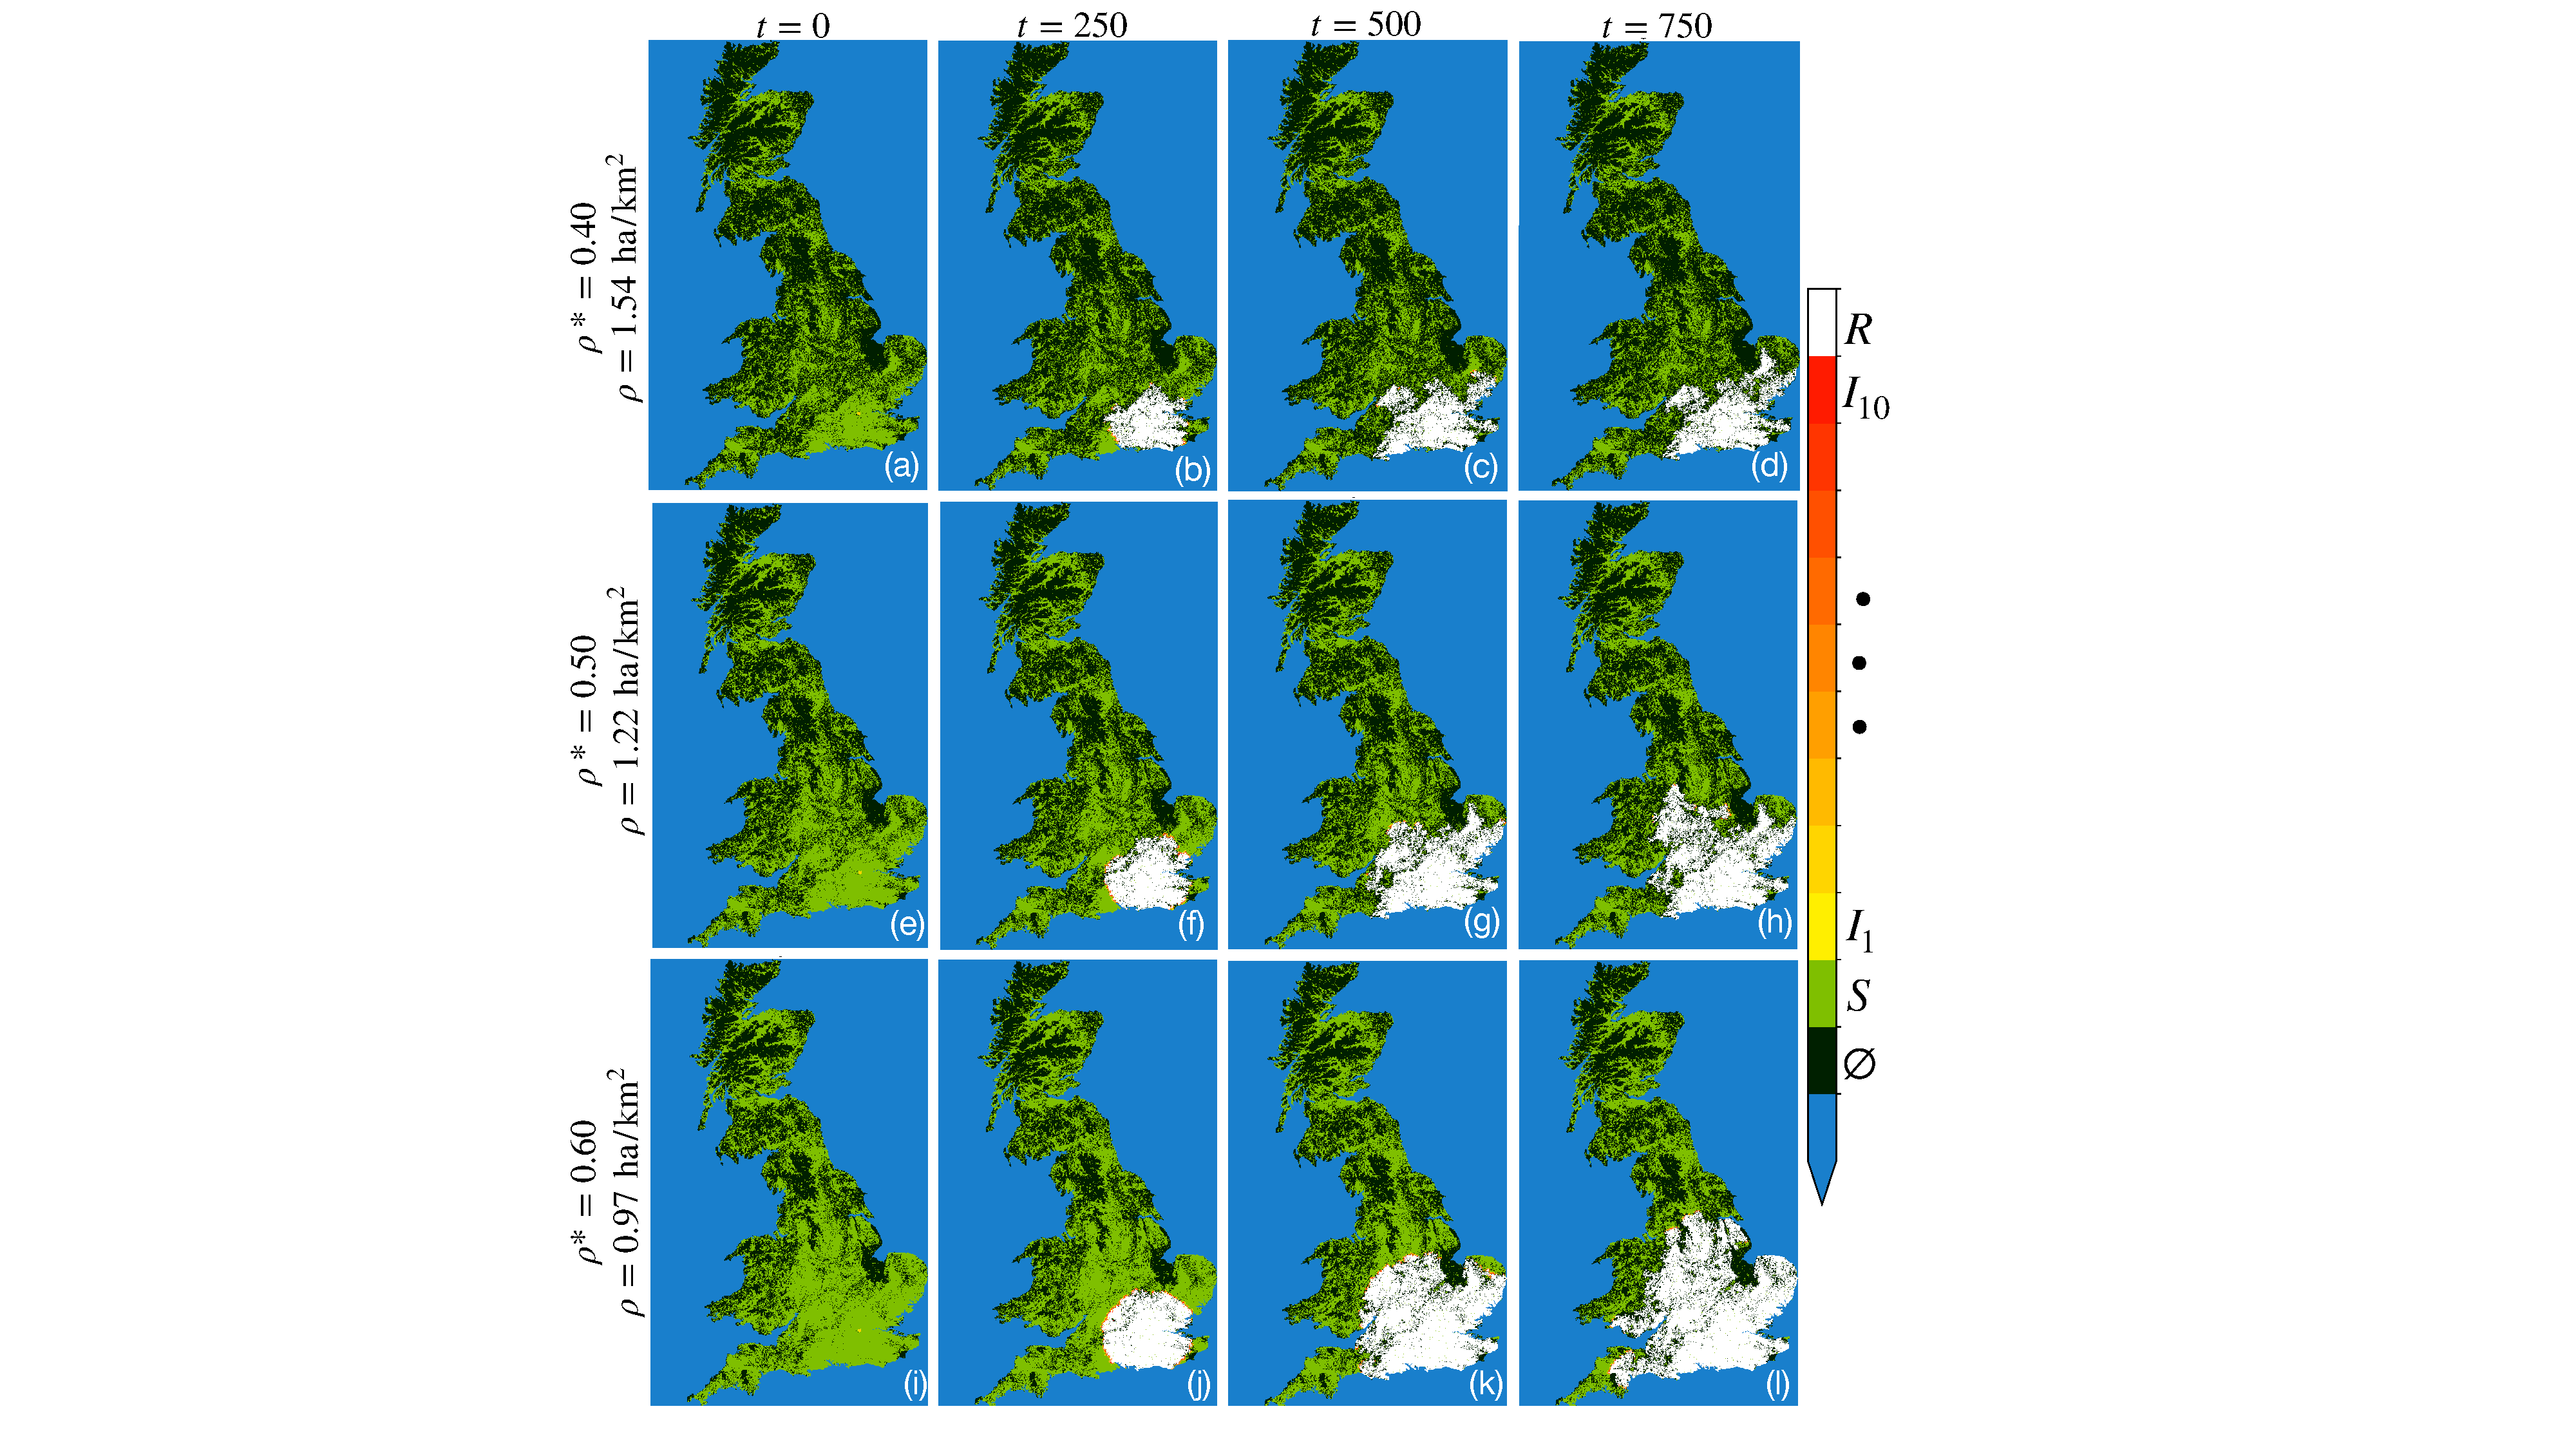
\includegraphics[scale=0.490]{chapter4/figures/figure4.pdf}
    \caption{The simple lattice model running on a binary-valued Oak domain with infectivity $\beta=0.25$ for three variations of effective density $\rho^*$.}
    \label{fig:ch4_uk_spread}
\end{figure}

Using the effective density ($\rho^{*}$), defined in Eq (\ref{eq:rho_eff}), a set of %
binary-valued domains can be initialised from an arbitrarily chosen thresholds of abundance %
canopy cover ($\rho$). %
Figure \ref{fig:ch4_uk_spread} shows the domain that results from three variations of effective density $\rho^{*} \in [0.40, 0.50, 0.60]$, the corresponding thresholds of abundance canopy cover shown below. %
The SLM is projected onto the map as allowed to evolve indefinitely until pathogen-extinction. %
Figure \ref{fig:ch4_uk_spread} shows slices through four time-steps. %

From panels (a) (e) and (i), the differences in the domain density are apparent\textemdash larger values of abundance-threshold produce lower density maps. %
For all effective densities, the initial source of infection was planted in the south where canopy cover is most dense. %
The pathogen then initially progresses through the domain, $0<t<250$, unimpeded by a low number of insusceptible regions. %
Panels (f) and (j) show the how the process volved in a uniform manner showing to density is above the threshold for propagation. %
At $t=250$, panel (b) shows pathogen progression inhibited by a barrier of insusceptible patches. %


Previously, density was uniform in all directions. %
Now however, heterogeneity unevenly distributes susceptible patches of land. %
This has implications for the pathogens evolution and spread. %
As discussed in Chapter \ref{chapter:SLM}, the critical density for propagation is $\rho_c\sim 0.60$ and therefore propagation on the heterogeneous domain will result if the`\textit{local}' density satisfies $\rho>\rho_c$. %
This is true for Figure \ref{fig:ch4_uk_spread} around the initial source of infection. %
In panels (c) and (d) we can identify a centralised region in Great Britain, approximately extending from Oxford to Buckinghamshire where density is below the threshold. 
This results in pathogen-extinction just beyond $t=750$. %

Figure \ref{fig:ch4_uk_spread} hints towards clusters in the domain through which local densities are large enough to support an epidemic. %
For a domain of arbitrary density, consider two distinct clusters where local densities are above threshold, $C_1$ and $C_2$, with two lattice sites $p\in C_1$ and $q\in C_2$. %
Then $p \neq q$. However, small increases in $\rho^{*}$ have the potential to radically change the scale of epidemic impact by opening up a small number of susceptible patches such that $p=q$. %
This motivates an understanding of the relationship between $\rho^*$, $\beta$ and the final epidemic size. %
This can be summarised by the mortality ratio $\chi$, as defined in Eq (\ref{eq:epi_impact}). %

In this domain-configuration, percolation is ill-defined because there is now no notion of spatial extent between boarders as previously defined for the square lattice. %
Small changes in the epicenter and initial conditions can also can have large impacts on the progression of disease. %
Additionally, more noise and stochasticity is introduced to the time-series showing disease progression, which makes velocity-based metrics such as Eq (\ref{eq:vel_eff_r}) harder to use. %
In the heterogeneous domain, the most intuitive and informative metric to employ is the mortality ratio $\chi$. %

For this reason, it makes sense to investigate epidemic-impact as a function of epicenter-location. %
To do this, we employ the ensemble-averaging method shown in Figure \ref{fig:uk-spatial-risk} for different values of effective density and infectivity. %

\begin{figure}
    \centering
    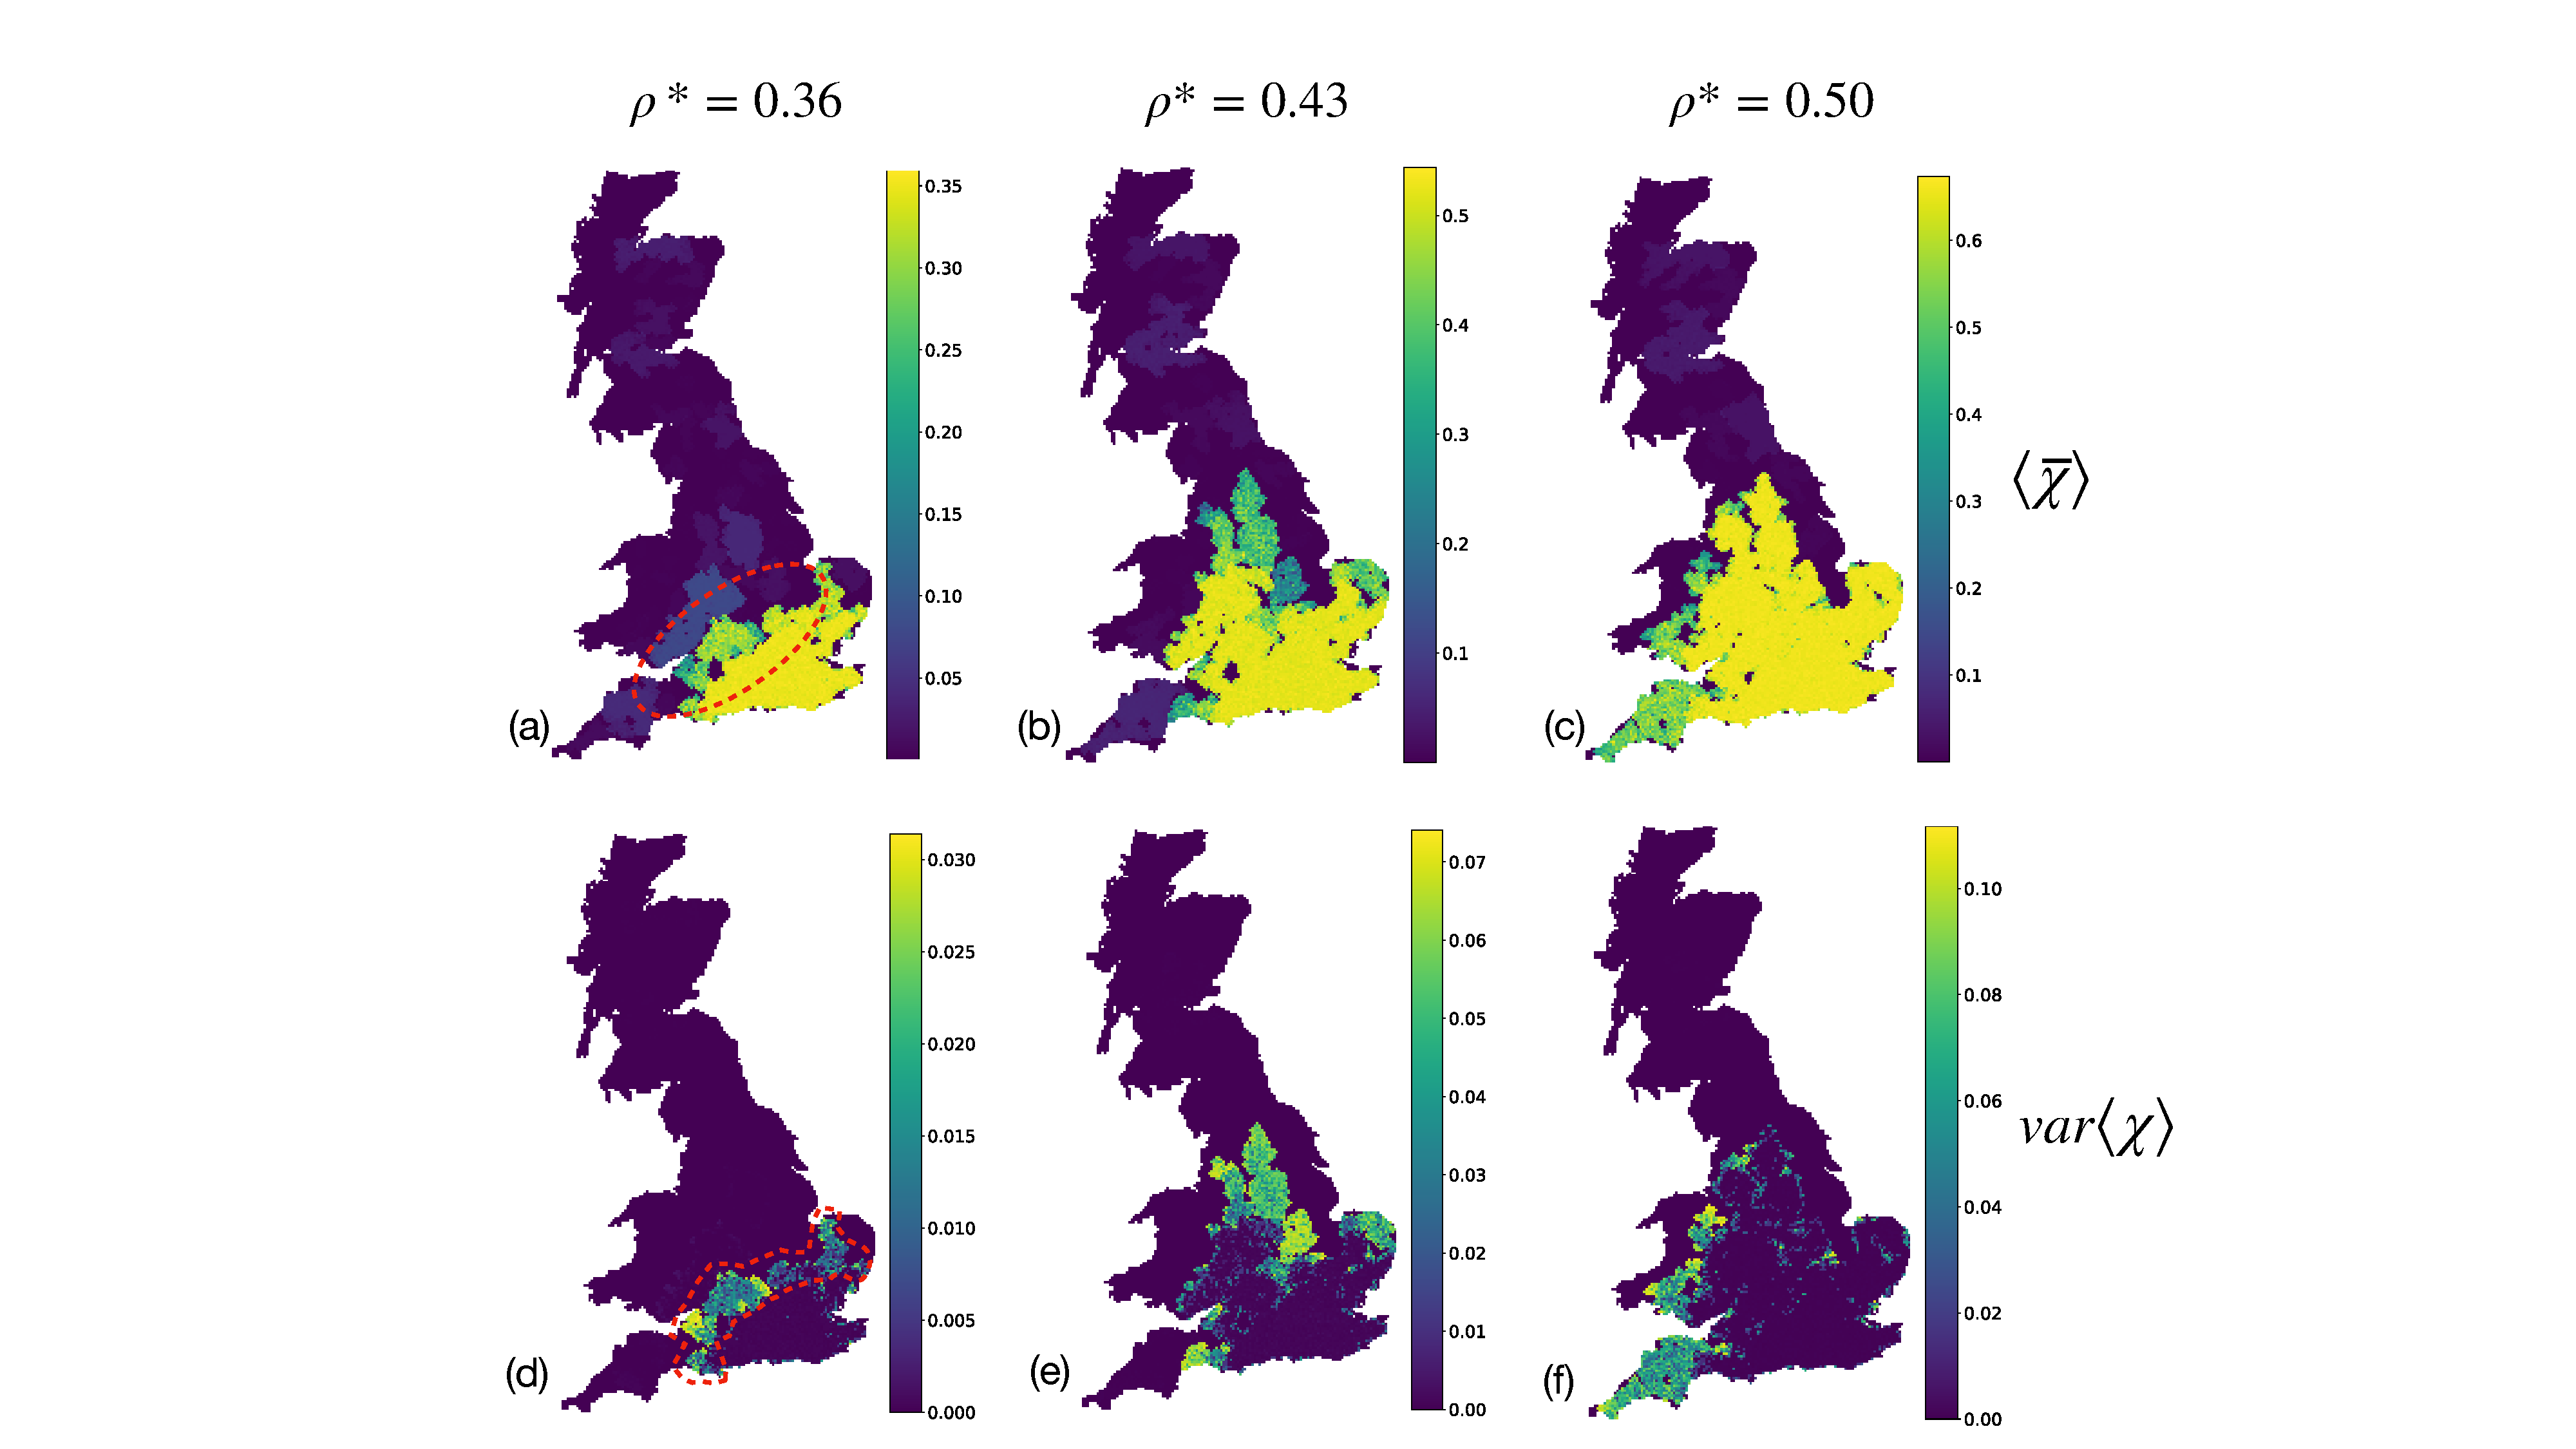
\includegraphics[scale=0.4]{chapter4/figures/figure5.pdf}
    \caption{Spatial phase showing ensemble statistics over the oak data-set for three variations of density threshold $\phi(\rho): \rho \in [0.37, 0.43, 0.50]$ and fixed infectivity $\beta=0.25$. (a-c) The ensemble mean of mortality ratio $\chi$ measured for each pixel epicenter. The dotted red circle in Fig (a) shows two neighbouring susceptible regions. (d-f) Ensemble variance over $\chi$. The dotted shape in (d) highlights an unstable region of high variance and uncertainty separating two susceptible areas of the population in Fig (a).}
    \label{fig:oak-spatial-ensemble}
\end{figure}

The spatially-iterated and ensemble-averaged method is applied to the Oak data-set, shown in Figure \ref{fig:oak-spatial-ensemble}. %
Panels (a-c) show the mortality ratio $\big\langle \overline{\chi} \big\rangle$ indicated by the colour bar for three different effective densities (conveniently chosen for the purposes of demonstration). %
For a given epicenter, variations of the epidemic-scale were seen between successive simulations. %
Thus, the bottom row (d-f), show the variance for each epicenter's ensemble, $\langle \chi_{i,j} \rangle$. %

As expected, increases in the effective density $\rho^*$ yield a higher epidemic-impact, as shown by the magnitude of successive colour bars % JS_colours represent what scale?
and expansive growth of susceptible clusters\textemdash shown in yellow. %
The most notable feature in panels (a-d) is that the  emergence is from a centrally-located cluster. %
Spatial locations within the solid yellow region are all connected via Von Neumann neighbourhoods (see Chapter \ref{chapter:SLM}) and the mortality is approximately independent of epicenter. %
In panel (a), the spatial locations encircled in dashed red, highlight a region of instability which appears to separate two susceptible clusters. %

The mortality ratio was observed to fluctuate between simulations, this is captured by variance in panels (d-f). %
Panel (c), highlights the variance in epidemic outcome inside the region of instability of panel (a). %
Panels (e) and (f) are similar, both showing variance only at the edges of one centrally located susceptible region. %
Plotting spatial variance captures epidemic uncertainty in the toy-model. %

Figure \ref{fig:oak-spatial-ensemble} fails to display any information about how far an epidemic is likely to propagate. %
This could be captured by the correlation function, see Section \ref{section:universality}. %
An alternative simplified representation can be captured by ensemble-averaging the maximum distance reached by the pathogen, %
shown in Appendix \ref{a:slm_heterogeneous}. %
In general, there are a variety of metrics that could be used to capture various aspects of an epidemic. %
Table \ref{tab:metrics} shows all metrics that were considered along with the information they provided. %

\begin{table}[h!]
  \begin{center}
    \begin{tabular}{l|c|c|r} % <-- Alignments: 1st column left, 2nd middle and 3rd right, with vertical lines in between
    \hline
      \textbf{Metric} & \textbf{Notation} & \textbf{Domain type} & \textbf{Information captured}\\
      \hline
      Percolation & $Pr(\rho,..)$ & Simple & Probability of epidemic \\
      Time & $t$ & Simple and GB-based & Time-scale of epidemic  \\
      Max distance & $d_{max}$ & Simple and GB-based & Spatial scale of epidemic\\
      Mean distance & $d_{av}$ & Simple and GB-based & Spatial scale of epidemic\\
      Median distance & $d_{med}$ & Simple and GB-based & Spatial scale of epidemic\\
      Mortality ratio & $\chi$ & Simple and GB-based & Scale of epidemic\\
      Radial velocity & $v(t)$ & Simple and GB-based & Rate of disease progression \\
      $COM$ velocity & $v_{CM}(t)$ & Simple and GB-based & Rate of disease progression\\
    \hline
    \end{tabular}
    \caption{A summary of applicable metrics to a given domain along with their uses.}
    \label{tab:metrics}
  \end{center}
\end{table}

\subsection{Heterogeneous phase diagram}

\begin{figure}
    \centering
    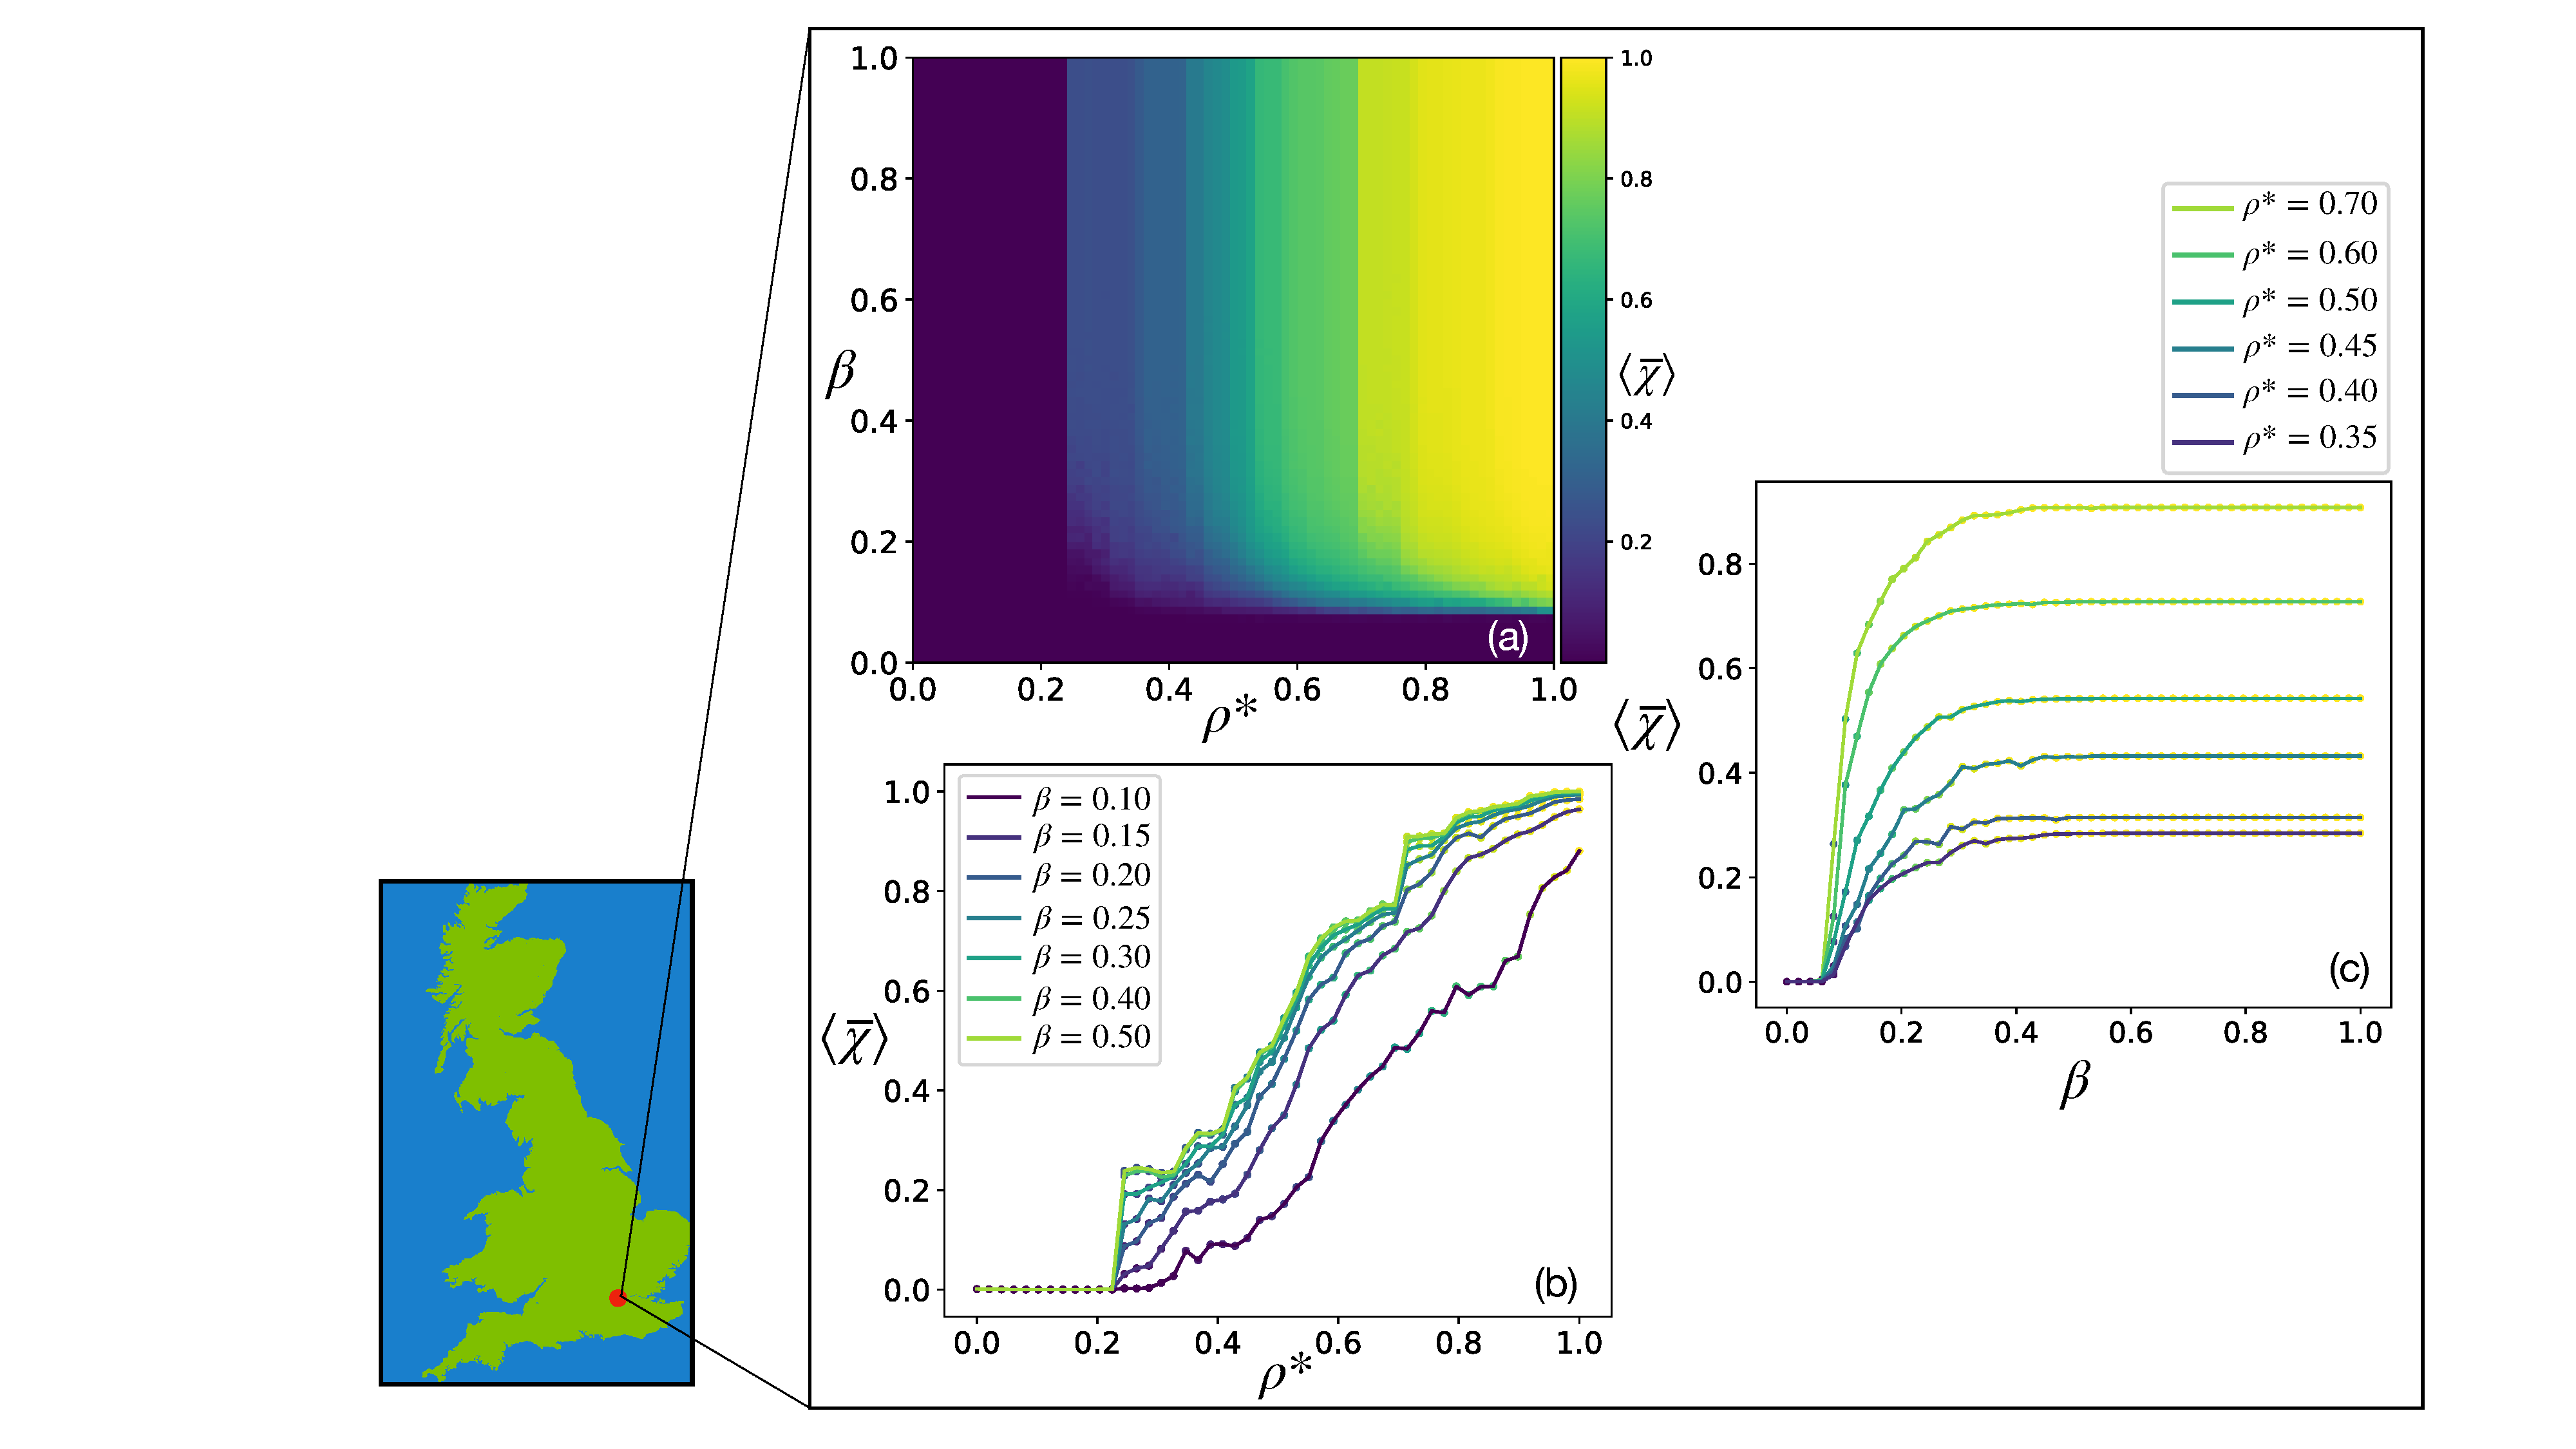
\includegraphics[scale=0.32]{chapter4/figures/figure6.pdf}
    \caption{The ensemble-averaged epidemic phase-space behaviour over a map of Great British Oak. Simulations were initialised from a single epicenter, shown in red. (a) The mortality ratio $\chi$, is shown over a two dimensional parameter space of $\rho^*$  and $\beta$. (b) The mortality ratio is found over $\rho^{*}$ for different values of infectivity (c) The mortality ratio is found over infectivity $\beta$ for different values of effective density $\rho^{*}$.}
    \label{fig:heterogeneous-phase-space}
\end{figure}

% JS_ This is an arrogant statement because it suggests you are being lazy, refusing to argue  what insight an Analytical approach reveals
 It is both computationally intractable, and superfluous, to work out the phase-plane diagram for every potential source of infection in the domain. %
 As such, only a single epicenter was considered\textemdash if required % JS_ under what circumstances would it be required? What if your Examiners' find a flaw and and argue you are missing something obvious?
this could easily be extended to a small number of different epicenters. %
Figure \ref{fig:heterogeneous-phase-space} shows the ensemble-averaged epidemic phase space of the SLM when projected onto the heterogeneous map of Great British Oak canopy data. %
The Parameter sweeps from $\rho^{*}$ and $\beta$ both were considered. %
% JS_ so now you are considering  phase-space
The phase-space behaviour demonstrates multiple discontinuities and sharp increases in $\chi$ for certain combinations of $\rho^{*}$ and $\beta$. %
This occurs in stark contrast to the SLM phase-diagram for a random homogeneous domain. %
Figure \ref{fig:heterogeneous-phase-space}(a) reveals a large asymmetry between $\rho^*$ and $\beta$ as more discontinuities appear when $\rho^*$ is increased. %
This behaviour is highlighted in Figure \ref{fig:heterogeneous-phase-space}(b) as slices through the parameter space of $\beta$ are plotted over a one-dimensional parameter space of $\rho^*$. %

Figure \ref{fig:heterogeneous-phase-space}(c) details how variations of $\rho^*$ effect the model behaviour through $\beta$-space. %
A minimum infectivity of $\beta\sim0.10$ can be seen, below which no propagation is observed. %
This is identical behaviour to the SLM evolution on a uniform domain. %
Increases in $\beta$ incur fewer discontinuities compared to increases in $\rho^*$, as evidenced by smoother curves. %

The mortality ratio is independent of infectivity beyond $0.30 \lessapprox \beta$. %
This can be understood as follows: consider a domain with fixed density $\rho^*$ and $\beta=0.30$. %
The probability of a susceptible patch remaining susceptible when it encounters an infected neighbour is given by Eq (\ref{eq:pr_s_s}) as $Pr(S \rightarrow S) = (1 - 0.30)^{10} = 0.03$. %
Thus, on average the pathogen transmits successfully to susceptible neighbours with probability $Pr=0.97$. %
If the epicenter happened to belong to a cluster of size $100$, thus on average just three patches remain susceptible. %
In this case therefore, most patches in the cluster become infected and further increases in $\beta$ do not effect the % 
outcome\footnote{Increasing the infectivity to $\beta=0.40$ yields a $Pr(S \rightarrow S) = 0.006$, this would lead to negligible changes in the final epidemic size\textemdash however, the rate of progression would be faster.} of $\chi$. %
For $0.30 \lessapprox  \beta$, only increases to the domain density has the potential to raise the final epidemic size, %
this is indicated by the increases in the height of the curves in Figure \ref{fig:heterogeneous-phase-space}(c). %


\section{Chapter summary}

% Having established the SLM from first principles, the initial discussion of early warning %
% signals conducted by \cite{OROZCOFUENTES201912} was revisited using an alternate framework. %
% % 
% We used the \textit{mean} time-series variance, opposed to the variance of the \textit{mean} %
% time-series, a \textit{channel} domain with cylindrical boundary conditions and a metric that %
% traced the center of infectious-mass over time. From this, we proceeded to capture early warning %
% signals over a two dimensional parameter space whilst mitigating any unwanted geometrical effects. %
% % JS_can you rewrite and explain this more carefully ?

% When %setting up? 
% defining the early warning framework, a detailed description of the ensemble-averaging process %
% was given that permitted an unbiased treatment of simulations. %
% In this way, early warnings %
% were detected prior to the epidemic regime. Interestingly, asymmetries % JS_define these properly
% in the detection of early %
%  signals lead to some insightful observations about the model. %
%  % JS_be clear what is insighful!
%  Differences between a high $\beta$ and low $\rho$, were observed when compared against a low $\beta$ %
%  and high $\rho$ regime. For a high $\beta$ and low $\rho$ regime, early warning signals were detected %
%  further away from the epidemic regime. % JS_ explain further
%  In contrast, early warning signals for a low $\beta$ and high $\rho$ regime were only %
%  observable immediately before epidemic transition, although the variance spike was larger. %

% From these findings we may conjecture how it would be easier or harder to detect and prevent %
% either: a pathogen with infectivity on the verge of epidemic, or a region of hosts just below %
% the critical density. % JS_How dow these comment help you interpret other research?
% This could apply to a variety of systems in which environmental factors act to tip the pathogen %
% spread over the threshold for epidemic. % % JS_Can you explain what they are?

% Problematically however, the spread of disease through real systems cannot be ensemble averaged. %
% It therefore remains a speculative matter to consider how applicable this framework could be to %
% real landscapes and pathological systems. Early warning signals would be hard to resolve accurately in %
% practice due to various factors, including the cryptic nature of infestations, %
% long-ranged dispersal and more generally an insufficient knowledge of infected symptomatic hosts. %
% This re-investigation thus remains abstract and more work would need to be conducted before %
% accurate results can be established. %

In this chapter, the SLM operating on a realistic heterogeneous Oak tree canopy data has been considered as source of abundance. %
The units given were hectares of canopy cover per kilometer-squared $\mathrm{ha/km^2}$. %
The data source, given by \cite{hill.data}, was continuous and therefore incompatible with SLM %
when taken at face-value. % 
To account for this, we introduced an effective density parameter $\rho^*$ predicated on an %
arbitrarily chosen threshold value $\rho\ \mathrm{ha/km^2}$\textemdash defined in Eq (\ref{eq:rho_eff}). %
Where the abundance threshold $\rho$ represents a percentage of cover and therefore can be likened to the SLM density-parameter. %

At this point in the investigation, introducing an additional parameter $\rho^*$ is undesirable. %
In practice, ascertaining the threshold value $\rho$ for real host-pathogen interactions would add to the complexity and non-trivial to parse with the current toy-model. %
There were a few options to pre-possess the data that could have mitigated the introducing of an arbitrarily chosen threshold. %
An alternative we did not explore, is to consider initialising a random homogeneous square lattice inside the pixel of the canopy cover data. %
Doing so would be trivial to implement as abundance represents a percentage cover per unit of landmass, therefore reformulating the domain would simply involve multiplying the data by a factor $0.01$. %

Recasting the abundance data into a series of random-homogeneous domains exposes problems. %
Firstly, initialising a square lattice inside each pixel would incur a significant computational cost. %
Secondly, and most crucially, considering the numerical value of highest abundance patch we considered, $10\mathrm{ha/km^2}$ would translate into an SLM lattice density of just $0.10$, which  is far below the threshold $\rho_c \sim 0.60$ we computed in Chapter \ref{chapter:SLM}.%
Simply put, the mean distance between trees is too far and would not support simplified the NN interactions we have considered so far. 

Combining the SLM with the realistic data-source is a essential exercise as it revealed the SLM is the wrong model when considering large, realistic landscapes where the mean density (i.e. averaged over $1km^2$) is far below the threshold for propagation. %
This is not to say SLM would be useful for dense pockets of forest, both commercial plantations and natural, germane to small-scales. %
However, as we are motivated here by understanding large epidemics that spread over national-scales, so a change to the model must be made. 

To account for the low density of trees when smoothed over the landscape, we will now move towards a non-local model of spread describing pathogen dispersal. %
In this paradigm, transmission between trees can occur over larger length-scales and permit the spread over lower tree-densities. %
This is more reflective with the spread observed in Nature and has the desired effect of making the abundance threshold $\rho$ redundant. %
Such a scenario  allows the model to be directly informed by a realistic data-source of canopy coverage.
\newpage
